%----------------------------------------------------------------------------------------
%	PACKAGES AND OTHER DOCUMENT CONFIGURATIONS
%----------------------------------------------------------------------------------------

\documentclass[11pt,fleqn]{book} % Default font size and left-justified equations

\usepackage[top=3cm,bottom=3cm,left=3.2cm,right=3.2cm,headsep=10pt,letterpaper]{geometry} % Page margins

\usepackage{xcolor} % Required for specifying colors by name
\definecolor{ocre}{RGB}{52,177,201} % Define the orange color used for highlighting throughout the book

% Font Settings
\usepackage{avant} % Use the Avantgarde font for headings
%\usepackage{times} % Use the Times font for headings
\usepackage{mathptmx} % Use the Adobe Times Roman as the default text font together with math symbols from the Sym­bol, Chancery and Com­puter Modern fonts

\usepackage{microtype} % Slightly tweak font spacing for aesthetics

\usepackage[utf8]{inputenc}


\usepackage{epigraph}
\usepackage{wrapfig}
% Bibliography
\usepackage[style=alphabetic,sorting=nyt,sortcites=true,autopunct=true,babel=hyphen,hyperref=true,abbreviate=false,backref=true,backend=biber]{biblatex}
\addbibresource{bibliography.bib} % BibTeX bibliography file
\defbibheading{bibempty}{}


%----------------------------------------------------------------------------------------
%	VARIOUS REQUIRED PACKAGES
%----------------------------------------------------------------------------------------

\usepackage{titlesec} % Allows customization of titles

\usepackage{graphicx} % Required for including pictures
\graphicspath{{Pictures/}} % Specifies the directory where pictures are stored

\usepackage{wrapfig}

\usepackage{tikz} % Required for drawing custom shapes
\usepackage[T2A]{fontenc}
\usepackage[russian, romanian]{babel} % English language/hyphenation



\usepackage{enumitem} % Customize lists
\setlist{nolistsep} % Reduce spacing between bullet points and numbered lists

\usepackage{booktabs} % Required for nicer horizontal rules in tables

\usepackage{eso-pic} % Required for specifying an image background in the title page

\usepackage{keyval}
%----------------------------------------------------------------------------------------
%	MAIN TABLE OF CONTENTS
%----------------------------------------------------------------------------------------

\usepackage{titletoc} % Required for manipulating the table of contents

\contentsmargin{0cm} % Removes the default margin
% Chapter text styling
\titlecontents{chapter}[1.25cm] % Indentation
{\addvspace{15pt}\large\sffamily\bfseries} % Spacing and font options for chapters
{\color{ocre!60}\contentslabel[\Large\thecontentslabel]{1.25cm}\color{ocre}} % Chapter number
{}  
{\color{ocre!60}\normalsize\sffamily\bfseries\;\titlerule*[.5pc]{.}\;\thecontentspage} % Page number
% Section text styling
\titlecontents{section}[1.25cm] % Indentation
{\addvspace{5pt}\sffamily\bfseries} % Spacing and font options for sections
{\contentslabel[\thecontentslabel]{1.25cm}} % Section number
{}
{\sffamily\hfill\color{black}\thecontentspage} % Page number
[]
% Subsection text styling
\titlecontents{subsection}[1.25cm] % Indentation
{\addvspace{1pt}\sffamily\small} % Spacing and font options for subsections
{\contentslabel[\thecontentslabel]{1.25cm}} % Subsection number
{}
{\sffamily\;\titlerule*[.5pc]{.}\;\thecontentspage} % Page number
[] 


%----------------------------------------------------------------------------------------
%	MINI TABLE OF CONTENTS IN CHAPTER HEADS
%----------------------------------------------------------------------------------------

% Section text styling
\titlecontents{lsection}[0em] % Indendating
{\footnotesize\sffamily} % Font settings
{}
{}
{}

% Subsection text styling
\titlecontents{lsubsection}[.5em] % Indentation
{\normalfont\footnotesize\sffamily} % Font settings
{}
{}
{}
 
%----------------------------------------------------------------------------------------
%	PAGE HEADERS
%----------------------------------------------------------------------------------------

\usepackage{fancyhdr} % Required for header and footer configuration

\pagestyle{fancy}
\renewcommand{\chaptermark}[1]{\markboth{\sffamily\normalsize\bfseries\chaptername\ \thechapter.\ #1}{}} % Chapter text font settings
\renewcommand{\sectionmark}[1]{\markright{\sffamily\normalsize\thesection\hspace{5pt}#1}{}} % Section text font settings
\fancyhf{} \fancyhead[LE,RO]{\sffamily\normalsize\thepage} % Font setting for the page number in the header
\fancyhead[LO]{\rightmark} % Print the nearest section name on the left side of odd pages
\fancyhead[RE]{\leftmark} % Print the current chapter name on the right side of even pages
\renewcommand{\headrulewidth}{0.5pt} % Width of the rule under the header
\addtolength{\headheight}{2.5pt} % Increase the spacing around the header slightly
\renewcommand{\footrulewidth}{0pt} % Removes the rule in the footer
\fancypagestyle{plain}{\fancyhead{}\renewcommand{\headrulewidth}{0pt}} % Style for when a plain pagestyle is specified

% Removes the header from odd empty pages at the end of chapters
\makeatletter
\renewcommand{\cleardoublepage}{
\clearpage\ifodd\c@page\else
\hbox{}
\vspace*{\fill}
\thispagestyle{empty}
\newpage
\fi}
%----------------------------------------------------------------------------------------
%	Ceccc STYLES
%----------------------------------------------------------------------------------------
    \usepackage[tableposition=top]{caption}
    \usepackage{subcaption}
    \DeclareCaptionLabelFormat{gostfigure}{Desen #2}
    \DeclareCaptionLabelFormat{gosttable}{Tabel #2}
    \DeclareCaptionFormat{myformat}{\fontsize{6}{10}\selectfont#1#2#3}
    
    \DeclareCaptionLabelSeparator{gost}{~---~}
    \captionsetup{labelsep=gost}

    \captionsetup[figure]{labelformat=gostfigure,format=myformat}
    \captionsetup[table]{labelformat=gosttable}
    \renewcommand{\thesubfigure}{\asbuk{subfigure}}
%----------------------------------------------------------------------------------------
%	THEOREM STYLES
%----------------------------------------------------------------------------------------

\usepackage{amsmath,amsfonts,amssymb,amsthm} % For math equations, theorems, symbols, etc

\newcommand{\intoo}[2]{\mathopen{]}#1\,;#2\mathclose{[}}
\newcommand{\ud}{\mathop{\mathrm{{}d}}\mathopen{}}
\newcommand{\intff}[2]{\mathopen{[}#1\,;#2\mathclose{]}}
\newtheorem{notation}{Notation}[chapter]

%%%%%%%%%%%%%%%%%%%%%%%%%%%%%%%%%%%%%%%%%%%%%%%%%%%%%%%%%%%%%%%%%%%%%%%%%%%
%%%%%%%%%%%%%%%%%%%% dedicated to boxed/framed environements %%%%%%%%%%%%%%
%%%%%%%%%%%%%%%%%%%%%%%%%%%%%%%%%%%%%%%%%%%%%%%%%%%%%%%%%%%%%%%%%%%%%%%%%%%
\newtheoremstyle{ocrenumbox}% % Theorem style name
{0pt}% Space above
{0pt}% Space below
{\normalfont}% % Body font
{}% Indent amount
{\small\bf\sffamily\color{ocre}}% % Theorem head font
{\;}% Punctuation after theorem head
{0.25em}% Space after theorem head
{\small\sffamily\color{ocre}\thmname{#1}\nobreakspace\thmnumber{\@ifnotempty{#1}{}\@upn{#2}}% Theorem text (e.g. Theorem 2.1)
\thmnote{\nobreakspace\the\thm@notefont\sffamily\bfseries\color{black}---\nobreakspace#3.}} % Optional theorem note
\renewcommand{\qedsymbol}{$\blacksquare$}% Optional qed square

\newtheoremstyle{blacknumex}% Theorem style name
{5pt}% Space above
{5pt}% Space below
{\normalfont}% Body font
{} % Indent amount
{\small\bf\sffamily}% Theorem head font
{\;}% Punctuation after theorem head
{0.25em}% Space after theorem head
{\small\sffamily{\tiny\ensuremath{\blacksquare}}\nobreakspace\thmname{#1}\nobreakspace\thmnumber{\@ifnotempty{#1}{}\@upn{#2}}% Theorem text (e.g. Theorem 2.1)
\thmnote{\nobreakspace\the\thm@notefont\sffamily\bfseries---\nobreakspace#3.}}% Optional theorem note

\newtheoremstyle{blacknumbox} % Theorem style name
{0pt}% Space above
{0pt}% Space below
{\normalfont}% Body font
{}% Indent amount
{\small\bf\sffamily}% Theorem head font
{\;}% Punctuation after theorem head
{0.25em}% Space after theorem head
{\small\sffamily\thmname{#1}\nobreakspace\thmnumber{\@ifnotempty{#1}{}\@upn{#2}}% Theorem text (e.g. Theorem 2.1)
\thmnote{\nobreakspace\the\thm@notefont\sffamily\bfseries---\nobreakspace#3.}}% Optional theorem note

%%%%%%%%%%%%%%%%%%%%%%%%%%%%%%%%%%%%%%%%%%%%%%%%%%%%%%%%%%%%%%%%%%%%%%%%%%%
%%%%%%%%%%%%% dedicated to non-boxed/non-framed environements %%%%%%%%%%%%%
%%%%%%%%%%%%%%%%%%%%%%%%%%%%%%%%%%%%%%%%%%%%%%%%%%%%%%%%%%%%%%%%%%%%%%%%%%%
\newtheoremstyle{ocrenum}% % Theorem style name
{5pt}% Space above
{5pt}% Space below
{\normalfont}% % Body font
{}% Indent amount
{\small\bf\sffamily\color{ocre}}% % Theorem head font
{\;}% Punctuation after theorem head
{0.25em}% Space after theorem head
{\small\sffamily\color{ocre}\thmname{#1}\nobreakspace\thmnumber{\@ifnotempty{#1}{}\@upn{#2}}% Theorem text (e.g. Theorem 2.1)
\thmnote{\nobreakspace\the\thm@notefont\sffamily\bfseries\color{black}---\nobreakspace#3.}} % Optional theorem note
\renewcommand{\qedsymbol}{$\blacksquare$}% Optional qed square
\makeatother

% Defines the theorem text style for each type of theorem to one of the three styles above
\newcounter{dummy} 
\numberwithin{dummy}{section}
\theoremstyle{ocrenumbox}
\newtheorem{theoremeT}[dummy]{Theorem}
\newtheorem{problem}{Problem}[chapter]
\newtheorem{exerciseT}{Exercise}[chapter]
\theoremstyle{blacknumex}
\newtheorem{exampleT}{Example}[chapter]
\theoremstyle{blacknumbox}
\newtheorem{vocabulary}{Vocabulary}[chapter]
\newtheorem{definitionT}{Definition}[section]
\newtheorem{corollaryT}[dummy]{Corollary}
\theoremstyle{ocrenum}
\newtheorem{proposition}[dummy]{Proposition}

%----------------------------------------------------------------------------------------
%	DEFINITION OF COLORED BOXES
%----------------------------------------------------------------------------------------

\RequirePackage[framemethod=default]{mdframed} % Required for creating the theorem, definition, exercise and corollary boxes

% Theorem box
\newmdenv[skipabove=7pt,
skipbelow=7pt,
backgroundcolor=black!5,
linecolor=ocre,
innerleftmargin=5pt,
innerrightmargin=5pt,
innertopmargin=5pt,
leftmargin=0cm,
rightmargin=0cm,
innerbottommargin=5pt]{tBox}

% Exercise box	  
\newmdenv[skipabove=7pt,
skipbelow=7pt,
rightline=false,
leftline=true,
topline=false,
bottomline=false,
backgroundcolor=ocre!10,
linecolor=ocre,
innerleftmargin=5pt,
innerrightmargin=5pt,
innertopmargin=5pt,
innerbottommargin=5pt,
leftmargin=0cm,
rightmargin=0cm,
linewidth=4pt]{eBox}	

% Definition box
\newmdenv[skipabove=7pt,
skipbelow=7pt,
rightline=false,
leftline=true,
topline=false,
bottomline=false,
linecolor=ocre,
innerleftmargin=5pt,
innerrightmargin=5pt,
innertopmargin=0pt,
leftmargin=0cm,
rightmargin=0cm,
linewidth=4pt,
innerbottommargin=0pt]{dBox}	

% Corollary box
\newmdenv[skipabove=7pt,
skipbelow=7pt,
rightline=false,
leftline=true,
topline=false,
bottomline=false,
linecolor=gray,
backgroundcolor=black!5,
innerleftmargin=5pt,
innerrightmargin=5pt,
innertopmargin=5pt,
leftmargin=0cm,
rightmargin=0cm,
linewidth=4pt,
innerbottommargin=5pt]{cBox}

% Creates an environment for each type of theorem and assigns it a theorem text style from the "Theorem Styles" section above and a colored box from above
\newenvironment{theorem}{\begin{tBox}\begin{theoremeT}}{\end{theoremeT}\end{tBox}}
\newenvironment{exercise}{\begin{eBox}\begin{exerciseT}}{\hfill{\color{ocre}\tiny\ensuremath{\blacksquare}}\end{exerciseT}\end{eBox}}				  
\newenvironment{definition}{\begin{dBox}\begin{definitionT}}{\end{definitionT}\end{dBox}}	
\newenvironment{example}{\begin{exampleT}}{\hfill{\tiny\ensuremath{\blacksquare}}\end{exampleT}}		
\newenvironment{corollary}{\begin{cBox}\begin{corollaryT}}{\end{corollaryT}\end{cBox}}	

%----------------------------------------------------------------------------------------
%	REMARK ENVIRONMENT
%----------------------------------------------------------------------------------------

\newenvironment{remark}{\par\vspace{10pt}\small % Vertical white space above the remark and smaller font size
\begin{list}{}{
\leftmargin=35pt % Indentation on the left
\rightmargin=25pt}\item\ignorespaces % Indentation on the right
\makebox[-2.5pt]{\begin{tikzpicture}[overlay]
\node[draw=ocre!60,line width=1pt,circle,fill=ocre!25,font=\sffamily\bfseries,inner sep=2pt,outer sep=0pt] at (-15pt,0pt){\textcolor{ocre}{R}};\end{tikzpicture}} % Orange R in a circle
\advance\baselineskip -1pt}{\end{list}\vskip5pt} % Tighter line spacing and white space after remark
%----------------------------------------------------------------------------------------
%	EXpli ENVIRONMENT
%----------------------------------------------------------------------------------------

\newenvironment{expli}{\par\vspace{10pt}\small % Vertical white space above the remark and smaller font size
\begin{list}{}{
\leftmargin=25pt % Indentation on the left
\rightmargin=25pt}\item\ignorespaces % Indentation on the right
\makebox[-2.5pt]{\begin{tikzpicture}[overlay]
\node[draw=ocre!60,line width=1pt,circle,fill=ocre!25,font=\sffamily\bfseries,inner sep=2pt,outer sep=0pt] at (-15pt,0pt){\textcolor{ocre}{E}};\end{tikzpicture}} % Orange R in a circle
\advance\baselineskip -1pt}{\end{list}\vskip5pt} % Tighter line spacing and white space after remark
%----------------------------------------------------------------------------------------
%	SECTION NUMBERING IN THE MARGIN
%----------------------------------------------------------------------------------------

\makeatletter
\renewcommand{\@seccntformat}[1]{\llap{\textcolor{ocre}{\csname the#1\endcsname}\hspace{1em}}}                    
\renewcommand{\section}{\@startsection{section}{1}{\z@}
{-4ex \@plus -1ex \@minus -.4ex}
{1ex \@plus.2ex }
{\normalfont\large\sffamily\bfseries}}
\renewcommand{\subsection}{\@startsection {subsection}{2}{\z@}
{-3ex \@plus -0.1ex \@minus -.4ex}
{0.5ex \@plus.2ex }
{\normalfont\sffamily\bfseries}}
\renewcommand{\subsubsection}{\@startsection {subsubsection}{3}{\z@}
{-2ex \@plus -0.1ex \@minus -.2ex}
{.2ex \@plus.2ex }
{\normalfont\small\sffamily\bfseries}}                        
\renewcommand\paragraph{\@startsection{paragraph}{4}{\z@}
{-2ex \@plus-.2ex \@minus .2ex}
{.1ex}
{\normalfont\small\sffamily\bfseries}}

%----------------------------------------------------------------------------------------
%	HYPERLINKS IN THE DOCUMENTS
%----------------------------------------------------------------------------------------

% For an unclear reason, the package should be loaded now and not later
\usepackage{hyperref}
\hypersetup{hidelinks,backref=true,pagebackref=true,hyperindex=true,colorlinks=false,breaklinks=true,urlcolor= ocre,bookmarks=true,bookmarksopen=false,pdftitle={Title},pdfauthor={Author}}

%----------------------------------------------------------------------------------------
%	CHAPTER HEADINGS
%----------------------------------------------------------------------------------------

% The set-up below should be (sadly) manually adapted to the overall margin page septup controlled by the geometry package loaded in the main.tex document. It is possible to implement below the dimensions used in the goemetry package (top,bottom,left,right)... TO BE DONE

\newcommand{\thechapterimage}{}
\newcommand{\chapterimage}[1]{\renewcommand{\thechapterimage}{#1}}

% Numbered chapters with mini tableofcontents
\def\thechapter{\arabic{chapter}}
\def\@makechapterhead#1{
\thispagestyle{empty}
{\centering \normalfont\sffamily
\ifnum \c@secnumdepth >\m@ne
\if@mainmatter
\startcontents
\begin{tikzpicture}[remember picture,overlay]
\node at (current page.north west)
{\begin{tikzpicture}[remember picture,overlay]
\node[anchor=north west,inner sep=0pt] at (0,0) {\includegraphics[width=\paperwidth]{\thechapterimage}};
%%%%%%%%%%%%%%%%%%%%%%%%%%%%%%%%%%%%%%%%%%%%%%%%%%%%%%%%%%%%%%%%%%%%%%%%%%%%%%%%%%%%%
% Commenting the 3 lines below removes the small contents box in the chapter heading
%\fill[color=ocre!10!white,opacity=.6] (1cm,0) rectangle (8cm,-7cm);
%\node[anchor=north west] at (1.1cm,.35cm) {\parbox[t][8cm][t]{6.5cm}{\huge\bfseries\flushleft \printcontents{l}{1}{\setcounter{tocdepth}{2}}}};
\draw[anchor=west] (5cm,-9cm) node [rounded corners=20pt,fill=ocre!10!white,text opacity=1,draw=ocre,draw opacity=1,line width=1.5pt,fill opacity=.6,inner sep=12pt]{\huge\sffamily\bfseries\textcolor{black}{\thechapter. #1\strut\makebox[22cm]{}}};
%%%%%%%%%%%%%%%%%%%%%%%%%%%%%%%%%%%%%%%%%%%%%%%%%%%%%%%%%%%%%%%%%%%%%%%%%%%%%%%%%%%%%
\end{tikzpicture}};
\end{tikzpicture}}
\par\vspace*{230\p@}
\fi
\fi}

% Unnumbered chapters without mini tableofcontents (could be added though) 
\def\@makeschapterhead#1{
\thispagestyle{empty}
{\centering \normalfont\sffamily
\ifnum \c@secnumdepth >\m@ne
\if@mainmatter
\begin{tikzpicture}[remember picture,overlay]
\node at (current page.north west)
{\begin{tikzpicture}[remember picture,overlay]
\node[anchor=north west,inner sep=0pt] at (0,0) {\includegraphics[width=\paperwidth]{\thechapterimage}};
\draw[anchor=west] (5cm,-9cm) node [rounded corners=20pt,fill=ocre!10!white,fill opacity=.6,inner sep=12pt,text opacity=1,draw=ocre,draw opacity=1,line width=1.5pt]{\huge\sffamily\bfseries\textcolor{black}{#1\strut\makebox[22cm]{}}};
\end{tikzpicture}};
\end{tikzpicture}}
\par\vspace*{230\p@}
\fi
\fi
}
\makeatother % Insert the commands.tex file which contains the majority of the structure behind the template

\begin{document}

%----------------------------------------------------------------------------------------
%	TITLE PAGE
%----------------------------------------------------------------------------------------

\begingroup
\thispagestyle{empty}
\AddToShipoutPicture*{\put(0,0){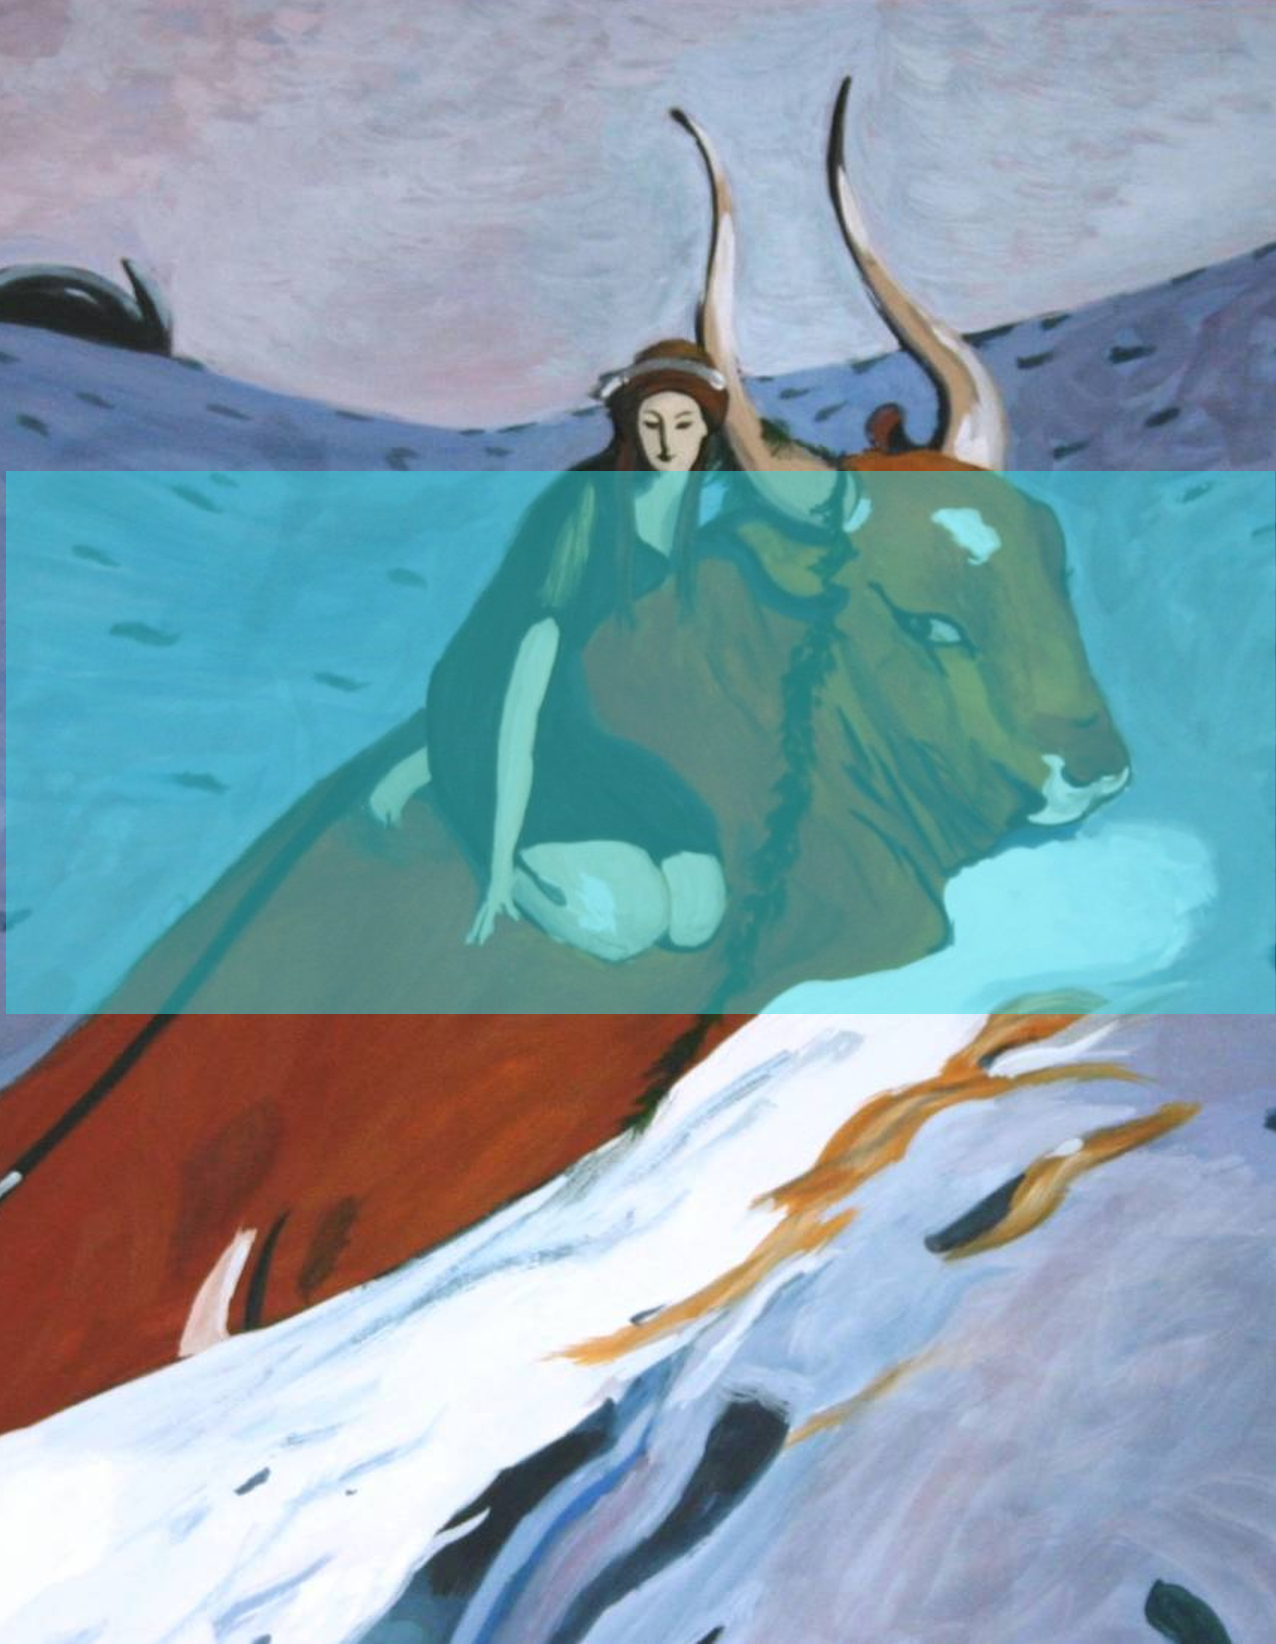
\includegraphics[scale=0.55]{europa1}}} % Image background
\centering
\vspace*{5cm}
\par\normalfont\fontsize{35}{35}\sffamily\selectfont
\textbf{ISTORIA EUROPEI}\\
{\LARGE Notiţe de curs}\par % Book title
\vspace*{1cm}
{\Huge Ghenadie Cabac}\par % Author name

\endgroup

%----------------------------------------------------------------------------------------
%	COPYRIGHT PAGE
%----------------------------------------------------------------------------------------

\newpage
~\vfill
\thispagestyle{empty}

\noindent Copyright \copyright\ 2015 Ghenadie V Cabac\\ % Copyright notice

\noindent \textsc{Universitatea de Stat "Alecu Russo" din Bălţi}\\

\noindent \textsc{www.usrarb.md}\\ % URL

\noindent O tentativă de conspect semantic\\ % License information
\noindent Versiunea 0.1\\ % Relise
\today
 



%----------------------------------------------------------------------------------------
%	TABLE OF CONTENTS
%----------------------------------------------------------------------------------------

\chapterimage{hist1e.jpg} % Table of contents heading image

\pagestyle{empty} % No headers

\tableofcontents % Print the table of contents itself

\cleardoublepage % Forces the first chapter to start on an odd page so it's on the right
\pagestyle{fancy} % Print headers again
\chapterimage{ddd.jpg} % Chapter heading image
\chapter{Întroducere}
\epigraph{Corrige praetertum, praesens rege, cerne futurum - Analizeaza trecutul, conducete de prezent, prevede viitorul }{Lucius Annaeus Seneca minor}
\section{Ce este istoria ?}\index{Ce este istoria ?}
\begin{wrapfigure}[16]{r}{0.2\linewidth} 
    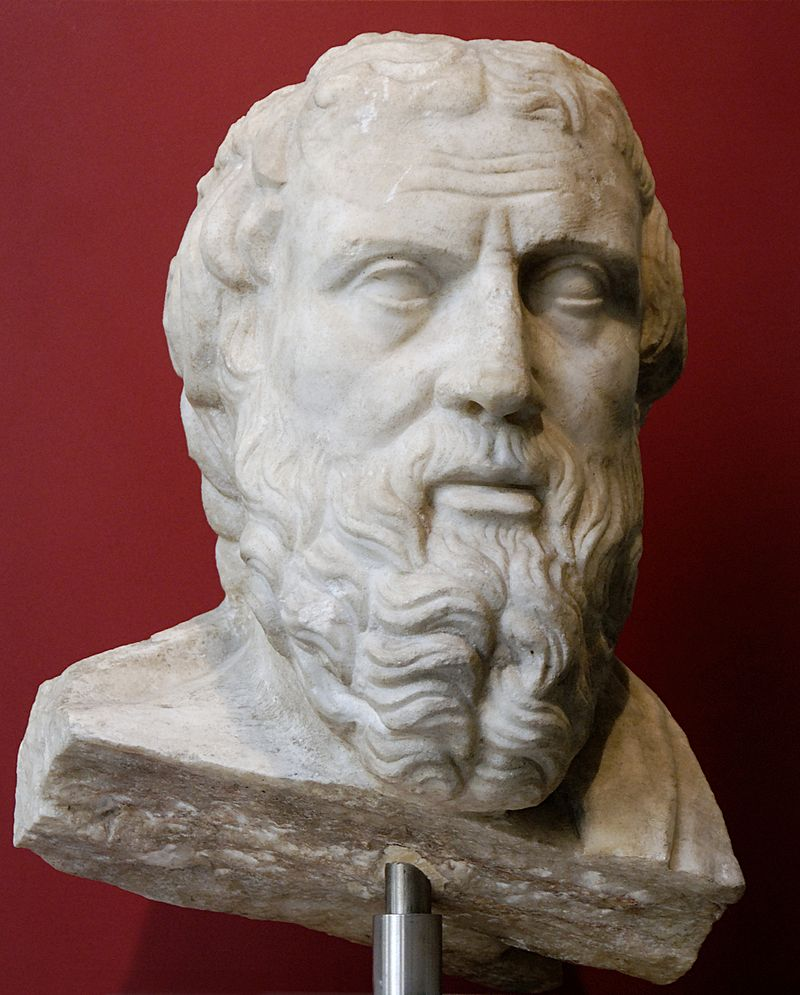
\includegraphics[width=0.27\textwidth]{herodot.jpg}
    \caption{Herodot. Marmură greacă, copie romană a unui original grec de la începutul secolului IV î.Hr.Porta Metronia, Roma.}
    \label{fig:pca}
\end{wrapfigure}
Interesul faţă de trecut este specific rasei umane. Acest interes este greu de explicat doar prin o curiozitate simplă. Faptul că omul însuşi  este o fiinţă istorică.  El se dezvoltă şi să schimbă în timp, fiind produsul a acestei dezvoltări.

Sensul originar al cuvântului "istorie" vine din vechea  greacă  ce insemna "anchetă", "recunoaştere", "înfiinţarea". În antichitate cuvântului "istoria" era folosit ca determinarea cunoştinţelor obţinute prin cercetări în general, adică nu numai despre evenimentele din trecut cum suntem deprinşi să folosim acest cuvînt astăzi. Astfel, Aristotel a folosit acest cuvînt în "Istoria animalelor". De asemenea, îl găsim în imnurile lui Homer, scrierile lui Heraclit şi în textul jurîmântului statului atenian.

Pentru o lungă perioadă de timp istoria nu este văzută ca o ştiinţă, ci  ca un compartiment al literaturii şi artei.Nu întîmplător în mitologia greacă, patronatul asupra istoriei era asigurat de una din muze Clio - o femeie tânără, cu o faţă înspirată, cu un papirus sau pergament în mînă. Numele  muzei Clio - este o derivată  a cuvîntului  grecesc "laudă".

\subsection{Herodot}
Personalitatea lui Herodot, datorită păstrării integrale a operei sale, ni se înfăţişează şi astăzi, aşa cum a fost acum două mii patru sute de ani în urmă, vie, iscoditoare, înclinată să cumpănească oamenii şi faptele lor. Cicero l-a numit pe Herodot "părintele istoriei". Caracterizarea lui Cicero cuprinde o bună parte de adevăr, fără pretenţia să-l identifice pe Herodot cu un adevăreat istoric. Herodot n-a fost altceva decât un cercetător harnic şi talentat, care - depăşind preocupările înguste ale logografilor - a trecut pentru prima oară la compoziţia istorică de proporţii vaste, axată pe un plan bine definit.

Faţă de lucrările predecesorilor săi, Herodot s-a avântat în Istorii la povestirea unui lung şir de evenimente din istoria Orientului şi a Greciei. Nucleul central al acestor evenimente care ţin de secolele al VI-lea şi al V-lea î.e.n., îl constituie războaiele greco-persane şi împrejurările care au dus la izbucnirea ciocnirii între perşi şi daci. Deoarece Herodot a scris cea dintâi istorie cu caracter universal în literatura greacă, afirmaţia lui Cicero apare justificată, caci nimeni până atunci nu se încumetase să închege povestea întâmplărilor din trecu într-o operă de sine stătătoare, străbătută de un fir conducător, şi prea puţini se interesaseră de istoria politică a statelor atunci existente.

\begin{wrapfigure}[11]{l}{0.3\linewidth} 
    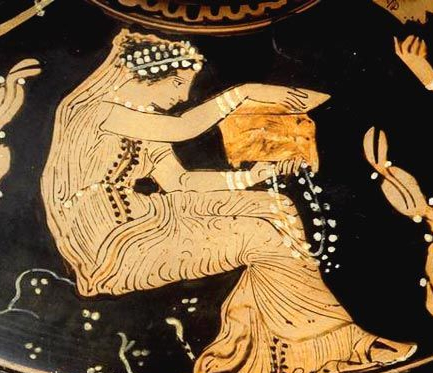
\includegraphics[width=0.27\textwidth]{Clio.jpg}
    \caption{Clio. Fragment de pe un vas grecesc 360 - 340  î.Hr.Porta Musee du Louvre, Paris, Franţa.}
    \label{fig:pca}
\end{wrapfigure}
Datele privitoare la viaţa lui Herodot sunt relativ puţine. Originar din Halicarnas, oraş în Caria colonizat de dorieni, şi integrat ulterior în aria civilizaţiei ioniene, Istoricul a văzut lumina zilei în răstimpul dintre expediţia lui Darius în Grecia (490 î.e.n.) şi ea a lui Xerxes (480 î.e.n.). Deşi n-a fost contemporanul marilor evenimente pe care le-a povestit, amintirea lor - păstrată pretutindeni în lumea elenică în cugetul celor mai vârstnici - i-a folosit cu prisosinţă ca să le descrie cât mai veridic şi plastic.

Din familia sa fruntaşă în Halicarnas, în afară de numele tatălui său, Lyxes, îl cunoaştem pe acela al lui Panyassis, ilustru poet epic, rudă apropiată cu Herodot (poate unchi ). La origine cariană, deşi de mult elenizată, familia lui Herodot se înrudea, în linie paternă, cu casa domnitoare din Halicarnas. Bucurându-se de sprijinul Persiei, casa domnitoare din Halicarnas nu se bucura, în schimb, de simpatia familiilor influente greceşti sau elenizate. Aşa se explică şi vrăjmăşia neîntreruptă arătată de familia lui Herodot tiranilor localnici, din care făcea parte însăşi celebra Artemisia, care l-a ajutat pe Xerxes în bătălia de la Salamina.

Educaţia primită de viitorul istoric al războaielor greco-persane s-a sprijinit pe concepţii de viaţă aristocratice, concepţii preţuite în cercurile influente din Ionia secolelor VI-V î.e.n Herodot a cunoscut îndeaproape creaţia epică şi cea a marilor poeţi lirici, înaintaşii lui, pe care-i şi citează adesea.

Din punct de vedere politic tânărul a participat la lupta dusă de familia sa împotriva tiranului Lygdamis al II-lea, fiul Artemisiei, stăpânitorul Halicarnasului din prima jumătate a secolului al V-lea.

Herodot se stinge din viaţă în jurul anului 425 î.e.n..

Istoriile lui Herodot, deşi în redactarea finală au un plan de concepţie bine definit, nu se înfăţişează ca o unitate desăvârşită. În mai mică măsură decât la epopeile homerice, s-au ivit şi pentru Herodot destule probleme în jurul redactării operei, din care cea mai de seamă rămâne întrebarea dacă autorul şi-a scris dintr-o dată opera, aşa cum o citim noi astăzi, sau a sudat într-un întreg povestiri istorice anterioare.

Subiectul întregii lucrări, care reprezintă, după mărturia autorului, o "cercetare personală", îl găsim enunţat de Herodot chiar la începutul cărţii I: "Herodot din Halicarnas înfăţişează aici rodul cercetărilor sale, pentru ca faptele oamenilor să nu pălească prin trecerea vremii, iar isprăvile mari şi minunate săvârşite şi de greci şi de barbari să nu fie date uitării ; printre altele va pomeni şi pricina pentru care aceştia s-au războit între olaltă".

Când a purces la adunarea materialului pentru vasta sa operă, Herodot a căutat să scrie o istorie cât mai bine documentată în raport cu posibilităţile epocii lui. Pentru aceasta a făcut întinse cercetări personale, a consultat monumente epigrafice şi arhive, s-a informat de la persoanele cele mai competente pe care le-a putut găsi. S.I. Sobolevski face următoarea clasificare pentru izvoarele folosite de Herodot: 1) observaţii personale făcute îndeosebi în cursul călătoriilor, însoţite de cercetări şi concluzii; 2) tradiţia verbală; 3)izvoare scrise.

Cu toată stăruinţa ce a depus-o, el n-a putut totuşi distinge cu fermitate perioada mitologică de cea istorică, nici graniţa dintre legendă şi adevăr. Anumite limite în cercetarea ştiinţifică de care n-a putut trece, limite comune în istoriografia contemporană lui, nu înseamnă că istoricul a fost lipsit de orice discernământ critic. Dimpotrivă, Herodot nu este un credul gata să accepte orice versiune fără să o cântărească, însă informaţia sa intelectuală şi pietatea religioasă l-au îndemnat adesea să accepte ca veridice informaţii care nu pot avea credit sau să tragă concluzii complet eronate.

Herodot obişnuieşte aproape întotdeauna să menţioneze izvorul informativ al faptelor relatate. Informaţia, uriaşă ca volum, pe care se sprijină compoziţia Istoriilor, se împarte în două categorii distincte: directă - fapte şi lucruri cunoscute sau văzute de istoric personal, indirectă - fapte şi lucruri aflate de la alţii. Concluzii deduse de Herodot însuşi pe calea raţionamentelor sunt comune ambelor categorii de informaţie; în majoritatea lor însă, ele nu pot sta în picioare, cum e cazul în cartea I, cap. CXCVI, de pildă, sau în cartea a II-a, cap. XXIV.

În istoria universală pe care a scirs-o Herodot, în munca uriaşă de unificare a părţilor ei componente nu putea lipsi o anumită concepţie asupra desfăşurării procesului istoric; diversitatea stadiilor orânduirii primitive şi sclavagiste pe care istoricul le-a luat în consideraţie l-au silit, la rândul lor, să reflecteze asupra dezvoltării societăţii omeneşti.\footnote{Herodot - Istorii, Ed. Ştiinţifică, 1961} 
\newpage

\section{Istoria ca ştiinţă}\index{Istoria ca ştiinţă}
\epigraph{Historia est Magistra Vitae}{Marcus Tullius Cicero}
After I arrived and had my first meeting with Pauline, she explained me a general idea of what she wanted and shared me some more papers (about multi-wavelenght studies), I read the information and came up with the objective.

\begin{itemize}
\item Find out a method to transform data from a high dimensional dataset (FITS cube or any other data arrangement) to a low dimensional understandable information (graphs, clusters).
\end{itemize}

This means that from multiple images with different wavelengths of the same target apply an algorithm to find the hidden patterns that lie hidden between them.

\section{Ştiinţele istorice}\index{Ştiinţele istorice}
Ok, here is where I explain from where this is going to start, at that time I just had a microcontrollers and engineering design course my mind was set completelly to find appplicable theories and create uselful things with them, which is the complete opposite of how astronomy works. First, there's no way to test an experiment with galaxies and most of the information is fuzzy and subjective (not all). The process of having an, let's say \emph{astronomy idea} is a result of applying all your physics knowledge and consider the \textbf{cosmological principle},
\begin{quote}
The (testable) assumption that the same physical laws that apply here and now also apply everywhere and at all times, and that there are no special locations or directions in the universe.
\end{quote}

That's how science is made, thinking and testing and thinking again, creating your own scientific method, comming up with hypothesis, learning what might work and what not, using your insticts. 

Well, before comming here I didn't think like that, it was just all about being super productive and thinking about doing robots and all kinds of devices with sensors. I had some experience programming in C/C++, no computer science backgound and I had never had an astronomy course.

This report was written in order to help someone to continue researching about data mining techniques applied in Astronomy, I explain how did I come up with the clustering techniques, my hypothesis, some tests and other ideas I have had, I hope this can help anyone and the research is continued. Anything you may need/questions do not hesitate to contact me, my e-mail address is: \emph{mrs.petzl@gmail.com}, also s part of my own documentation I created a GitHub page where you can download all the codes I programmed and find more information. The link to this page is: \url{https://github.com/LaurethTeX/Clustering}, from the \textsc{readme} file you can acces to all the pages, take your time to surf.
%------------------------------------------------

\subsection{References}\index{References}

Since I found so much good information about pretty much everything I wanted to know about, I will just create a remark and let you know where you can find more specific information about, just like below.


\begin{expli}
For more information about the cosmological principle, review Chapter 1: Why Learn Astronomy?, page 10, from \textbf{21st Century Astronomy}, \textit{Hester | Smith | Blumenthal | Kay | Voss}, Third Edition, 2010.
\end{expli}


%This statement requires citation \cite{book_key}; this one is more specific \cite[122]{article_key}.

\chapterimage{prehiste.jpg} % Chapter heading image

\chapter{Preistoria}
\epigraph{Şi a fost seară şi a fost dimineaţă: ziua întâi.}{Genesis 1.5}
\section{Răsăritul omenirii. Un milion de ani pînă la era noastră}
Soarele african strălucea peste savana, peste marginea verde a junglei şi crestele de nisip al văii Oldoway. Aici colo se vedeau turme de antilope şi girafe. Masivi ca nişte munţi hoinăreau rinoceri gigantici, care nu se temeau nici de stăpânii savanei - machairodzi (tigrii cu dinţi ca sabia) şi leii cavernelor. Şi undeva aici, în junglele şi savanele din Africa de Est, locuite de strîmoşii oamenilor, maimute Australopithecus, care la fel de abil usrcau în copaci şi mergeau pe două picioare pe pamant. Nu prea înalţi, pîr îndesat, pielea inchisa la culoare şi fălci puternice. Ei aveau arme teribile pentru alte animale - măciuca, lovitura căreia era la fel de puternică ca lovitura labei de leu. Măciuca a fost prima invenţie a maimuţelor pe drumul lor spre dominaţia mondială. Apoi au urmat suliţa şi focul, ce lea dat stăpînire peste savană. Fluturînd suliţe şi torţe, vînătorii mînau turmele de antilope înebunite de groază către prăpastie - unde vânătorii cei mai experimentati omorau animale rănite. Apoi, se făcea un foc, unde erau prăjite de întregu animalele vînate. Rupeau cu mâinile carnea fierbinte... Sătui, urcau în peşterele şi aţipeau pînă a doua zi, pînă la vînătoarea următoare. 
\begin{wrapfigure}[10]{r}{0.3\linewidth} 
    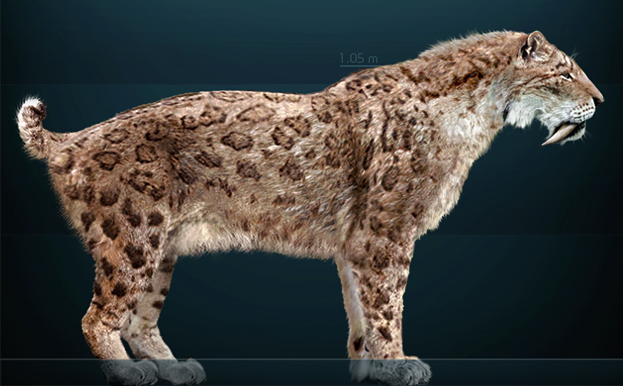
\includegraphics[width=0.4\textwidth]{mahaiord.jpg}
    \caption{Machairod (tigrul cu dinţi ca sabia) . Reconstrucţie grafică a Fatalis Smilodon bazat pe structurii osoase şi texte paleontologice.}
    \label{fig:pca}
\end{wrapfigure}

Nici rinocerii şi nici mamuţii uriaşi ce trăiau mai la nord nu puteu rezista turmele de maimuţe; cel mai temut duşman nu erau rinoceri sau leii, erau alte turme de maimuţe. În anii de foamete turmele vînau alte turme, toporele de piatră despicau craniile duşmanilor. Ca apoi câştigătorii, fluturând suliţe, ca de obicei, îi mînau pe cei învinşi în prăpastie. Ca întotdeauna, se făcea un foc şi se mînca prada, iar oasele învinşilor erau amesticate cu osele antilopelor vînate cîndva. 

Acest lucru a continuat din an în an, din secol în secol. Schimbarea climei, gheţarii care veneau de la nord, schimbarea întregii naturi au dus şi la schimbarea maimuţei; mîinile lor au devinit mai scurte, maxilarile mai mici şi capul a crescut în dimensiune. Australopithecus este substituit de Pithecanthropus,iar Pithecanthropus de Neanderthal, dar nu erau oamenii. Ele au rămas maimuţe - cu toate că s-au învăţat să se îmbrace în piei. Doar un miracol ar putea transforma o maimuţă într-un om. 
\subsubsection{Antropogeneza}
\epigraph{Triburile paleolitice au fost pline de tinereţe care nu se va mai întoarce, acea viaţă, energie şi putere pe care putem să ne o imaginăm cu greu.}{Joseph Henri Honoré Boex}

Preistoria constituie cea mai îndelungată perioadă din istoria umanităţii şi se înscrie, ca durată, de la primele manifestări ale prezenţei omului, atestate pe baza descoperirilor arheologice, până la descoperirea scrisului.

\begin{wrapfigure}[10]{l}{0.3\linewidth} 
    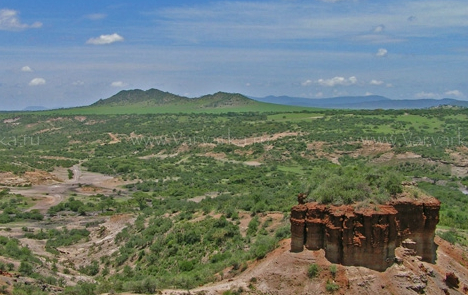
\includegraphics[width=0.3\textwidth]{oldoway.jpg}
    \caption{Valea Oldoway. Fotografie contemporană}
    \label{fig:pca}
\end{wrapfigure}
Istoria pune în prim plan geneza şi componenţa ei fundamentală, Omul. În timpul cuaternarului, în mai multe rânduri, s-au produs înaintări şi retrageri ale gheţarilor, corelate încă din 1874, de către J.Geikje, cu dezvoltarea culturilor paleolitice.

Antropogeneza studiază formarea şi dezvoltarea omului. Ea relevă trecerea omului din starea de animalitate în cea de umanitate, trecere condiţionată de trei coordonate esenţiale: starea bipedă, limbajul articulat şi gândirea. Locul şi data apariţiei omului pe Pământ este incertă.

Drumul spre sapientizare, respectiv către Homo Sapiens, a fost interpretat multă vreme din perspectiva evoluţionismului, evoluţia fiind considerată continuă şi ascendentă. Era contestată expresia biblică a genezei omului, într-o încercare de laicizare a gândirii, în două variante: fie omul se trage din maimuţă, fie sunt veri.

Descoperiri recente au pus în evidenţă şi alte posibilităţi de interpretare a genezei omului şi a raportului acestuia cu mediul geografic natural. Conform noii ipoteze, evoluţia este privită, în continuare în ascensiune, dar în spirală şi sinuoasă.

Dincolo de aceste ipoteze, un fapt este cert: omul a devenit o prezenţă activă într-un mediu  care, fără a-l favoriza în mod deosebit, nu i-a fost niciodată ostil.

Întemeiată pe studii etnografice asupra unor populaţii arhaice contemporane, ideea unei aşa-zise “vârste de aur” a umanităţii câştigă tot mai mulţi adepţi, lăsând în urmă, justificat în numeroase privinţe mitul omului neajutorat.

Pentru acest nivel de dezvoltare, persistenţa ideii de proprietate comună, absolută nu-şi mai are, nici ea, puncte de susţinere: delimitarea grupelor de vârstă, existenţa deosebirilor natural-biologice, statutul aparte, într-o comunitatea, al fiecărui membru al său, dezvăluie existenţa şi manifestarea simţului proprietăţii individuale.

În ceea ce priveşte începutul organizării sociale, trebuie regândită, din perspectivă, deosebirile dintre om şi lumea animală.

Direct sau indirect, mai mulţi factori au determinat fenomenul  răspândirii grupurilor umane pe Glob: schimbările geo-climatice, progresul tehnologic, capacitatea de adaptare a omului etc.

Dintr-o zonă restrânsă, între 1.800.000 - 900.000 este atestată o prezenţă generalizată a omului în întreaga Africă, Asia de sud, Europa de sud.

Aproximativ în acelaşi interval de timp (32.700 î.Hr.), grupe umane ating Australia.

America a fost şi ea populată prin strâmtoarea Behring, în timpul glaciaţiei Sartan (28.000-20.000 î.Hr.), în mai multe etape. Către neolitic sunt populate insulele Creta, Cipru şi Cicladele. Cu paleoliticul superior se constată un fenomen care îşi va pune amprenta asupra evoluţiei ulterioare a umanităţii: dezvoltarea mai accentuată a unor zone în raport cu altele care au evoluat tehnologic şi cultural mai puţin rapid.
\subsubsection{Dezvoltarea speciei umane}

\epigraph{Şi a zis Dumnezeu "Sa facem om după chipul şi dupa asemanarea noastră"}{Genesis 1.2}
Dezvoltarea omului din stamosii sai mai putin aratosi si inteligenti a avut loc in timpul ultimelor doua milioane de ani. Este probabil ca primul stadiu al acestei ramuri de evolutie organica, care a adus la ceea ce numim astazi Homo sapiens, sau omul care gandeste, sa fi inceput in Africa, in timpul pliocenului superior. In 1959, arheologul englez Louis Leakey a gasit in Africa de est resturile lui Zinjantropus, care se poate sa fi fost stra-stra-stra...bunicul nostru, al tuturor. Zinjantropus (numele inseamna omul est-african) a trait acum 1.750.000 ani si este cel mai vechi cioplitor de unelte de piatra pe care il cunoastem.

Fosilele lui australopitecus, omul-maimuta sud-african care a trait acum aproximativ 2.000.000 ani, au fost descoperite in 1920 de savantul englez Raymond Dart, impreuna cu arme de os si cu resturile animalelor ucise de el.

Din putinele urme de fosile descoperite reiese ca aceste fiinte cu aspect omenesc sau deplasat spre nord si spre est, raspandindu-se in toata Europa si Asia. In anul 500.000, pitecantropul traia pe insula Djawa si sinantropul in apropiere de actuala asezare a Peking-ului. Reprezentantii acestor doua genuri, care au disparut de mult, semanau foarte mult intre ei, ceea ce i-a facut pe antropologi sa-i includa intr-unul singur. Capacitatea lor craniana era de aproximativ 1000 centimetri cubi, in comparatie cu 1500 centimetri cubi, cat reprezinta cutia craniana a omului. Acesti indivizi, care erau destul de avansati pentru a-i putea considera stramosii nostri, aveau fruntea tesita si arcadele foarte pronuntate. Pitecantropul era familist, dar nu prea sociabil. El traia cu familia sa in padure si-si gasea adapost in pesteri. Se presupune ca se pricepea sa faca focul si sa-si construiasca obiecte simple si arme din lemn si piatra. Exista indicii ca acest tip de pre-om a trait si in Europa. Un maxilar gasit langa Heidelberg, in Germania se poate sa fi apartinut pitecantropului european.

Un stadiu mai avansat in evolutia omului il reprezinta omul de Neanderthal, ale carui ramasite se gasesc intr-un numar considerabil in Asia, Africa si Europa. Craniul sau era mai mare decat al pitecantropului, pe care il intreceau si ca indemanare. El era destul de scund si indesat, cu umerii incovoiati si genunchii usor indoiti, ca la maimutele de astazi. Fata sa era lata, fruntea joasa, cu arcadele proeminente; maxilarele semanau cu cele de animal, iar barbia era retrasa. Concurentul sau din alta ramura a rasei umane a fost omul de Cro-Magnon, numit astfel dupa pestera din apropierea micului sat Les Eyzies (sud-vestul Frantei), unde s-au gasit pentru prima oara resturile sale. Omul de Cro-Magnon era inalt brunet si chipes. Avea fruntea inalta, ceea ce dovedeste dezvoltarea partii frontale a creierului si barbia ascutita si proeminenta. Se pricepea foarte bine sa-si faca arme si sa vaneze, iar in timpul liber acoperea peretii cavernelor in care traia cu desene frumoase ale animalelor pe care le vana. Aceste desene pot rivaliza cu cele mai reusite picturi facute de oamenii moderni. E foarte probabil ca omul de Cro-Magnon stia sa vorbeasca si ca isi putea exprima emotiile si in muzica. Se prea poate sa fi existat o concurenta indarjita intre rasele Neanderthal si Cro-Magnon, cea din urma exterminand-o pe cea dintai. Astfel ajungem la omul de astazi. \footnote{O PLANETA NUMITA PAMANT, de George Gamow,Ed. Stiintifica, Buc. 1968, pag. 227 - 229} 

\subsection{Răsăritul omenirii. Patruzeci de mii de ani pînă la era noastră}
La fel strălucea peste savană soarele, la fel înverzeau copacii şi vîrfuri de munte străluceau la orizont.La fel se deplasau în lanţ pe câmpii vînătorii; dar în acest lanţ mergeau acum nu maimuţe dar oameni. Ei aveau aceleaşi topoare de piatră şi suliţe, dar nu arătau ca maimuţe. Ei erau înalţi, subţire şi vorbeau. Un miracol, unele mutaţie aleatoare au dus la faptul că a apărut primii oameni. 

Pentru un timp, oameni şi neanderthalienii trăiau unii lîngă alţii şi poate chiar se încălzeau la acelaş foc ca în peştera Tabun Cave din Palestina. Dar apoi sa întâmplat ceia ce trebuia să se întâmple: lipsa de alimente a generat între oameni şi neanderthalieni un război pe viaţă şi moarte. Gintele de oameni peste tot întâlneu neanderthalienii - stăpânii acestor locuri. Vînători mergînd în lanţ mînau neanderthalienii în prăpastie. Noile generaţii s-au mutat pese mişcau la sud, vest, est, avînd nevoie de noi terenuri. Ei urmăreau maimuţele izgoninindule în pădurii şi munţii. Peste zece mii de ani, cu neanderthalienii sa sfîrşit. Oameni au acaparat întreaga planeta. Doar unele popoare orientale, australieni şi ainu, au păstrat un mic amestec de sânge de Neanderthal - rezultatul amestecării învinşilor şi învingătorilor. 

A venit era de dominaţie a omului. Savanele, stepele şi tundra au fost împărţite între gintele de vânători. Deplasareaîndu-se mai departe spre nord, oamenii trecînd strâmtoarea încătuşată în geaţă au ajuns în America. Ei au populat un vast continent nou, pe care nu a călcat strămoşii lor- maimuţele. Chiar şi cei mai puternici nu au putut rezista noilor stăpîni ai lumii. Mamuţii uriaşi şi rinoceri au fost mînaţi în prăpastie la fel ca antilopele. Vînătorii dădeu foc la iarba şi soarteau la moarte tot ce era viu. Taberele lor au fost pline cu oasele de mii de bizoni şi cai. Mamuţii stângaci au fost sterşi de faţa pămîntului precum şi mastodonţi, cai americani şi zeci de alte specii. Oamenii ucideau animalele pentru a supravieţui. Ei deveneu mai mulţi la număr şi mai mult aveau nevoie de alimente. Ei populau pământul şi luau de la el tot ce puteau. Căutînd hrană - la fel ca şi strămoşii lor maimuţele - adunau plante comestibile. Apoi au învăţat cum să pescuiască, şi să se folosească de  năvod. Acum cincisprezece mii de ani, au inventat arcul ce a permis să vâneze păsări şi animale mici. Aceste descoperiri a fost o soluţie temporară, foamea se retrgea, ca apoi cînd populaţia crescu - se întorcea şi foametea. Anume ea impunea vînatul în lanţ a gintelor mai slabe. Arheologii astăzi găsesc în taberele vechi umane oase de mamuţi alături de oase de oameni. 

Omul era o parte a naturii - şi natura dicta legile ei crude.
\subsection{Omul şi natura}\index{Omul şi natura}
\epigraph{Populaţia este în mod inevitabil limitată de mijloacele de subzistenţă.}{Thomas Malthus}

Cu mult mai înainte decîtpînă cînd omul a devenit un stăpîn al planetei, leii dominau în savană. Leii, de asemenea, vânători  ca şi oamenii vînau în grup. După vânătoare împreună mâncau prada,  împreună aveau grijă de  puii şi trăiau într-o mare familie. Aveau teritoriul propriul şi luptau pentru el cu alte familii. Aceste lupte violente, mai devreme sau mai târziu sa încheiau cu moartea familiei.

Modul de viaţă a vînătorilor. Leoaica aduce în fiecare an mai mulţi puii care au nevoie de hrană; femeie dă viaţă copiilor care vor să mînînce. În ultimii ani, populaţia lumii a crescut cu doi la suta pe an, şi se poate presupune că numărul vînătorilor din acea perioadă creştea aproximativ la fel. În acest caz, ginta vînătorilor în jumătate de secol va creşte de 2,7 ori, iar pentru un secol - aproximativ de 7 ori. Vă puteţi imagina ce s-ar întîmpla în secolul următor? Peste două sute de ani numărul vînătorilor va creşte de 52 de ori, iar peste patru sute de anii - de 2700 de ori! Desigur, aceste nenumărate generaţii noi nu au suficientă mîncare şi un loc sub soare. Şi ei vor lupta pentru hrană - cu aceiaşi înverşunare ca şi leii.

Acestă forţă teribilă care îi mînă pe oamenii pe câmpul de luptă se numeşte \textbf{PRESIUNE DEMOGRAFICĂ}. Mai simplu, presiunea demografică - este foamea, adică mărimea învers proporţionară a consumului de alimente pe cap de locuitor. De exemplu, în Europa consumul de alimente este de două ori mai mare ca în India - aceasta înseamnă că presiunea demografică în India este de două ori mai mare, ceea ce înseamnă că India este în pericol constant de foamete şi războaie interne.

Imaginaţi-vă un teritoriu care aparţine unei ginţi de vînştori: păşiuni cu turme de animele ce pasc,pădurii pline de ciuperici şi rădăcini comestibile, un rîu bogat în peşte. Tot acest teritoriu, cu resursele sale alimentare - aceasta este  \textbf{NIŞA ECOLOGICĂ} a gintei. În cazul în care ginta creşte, ea preseză pereţii aceastei nişe, încercînd să o lărgească. Nişa ecologică poate fi extinsă prin unele invenţii, ca exemplu un harpon pentru un pescuit mai efecient  - invenţie care lărgeşte nişa ecologică, denumite \textbf{DESCOPERIRI FUNDAMENTALE}. Arcul, săgeţi otravite şi  nimimicirea gintei vecine, acapărarea pămînturilor lor  -  de asemenea este extinderea nişei ecologice. Măciuca, focul, suliţa, toporul de piatră, arcul - toate acestea au fost descoperiri fundamentale care au permis maimuţelor şi oamenilor să extindă nişa lor ecologică. Efectuarea acestor descoperiri, omul, în acelaşi timp, se schimba şi el. Oobiceiurile şi comportamentul  se complică spre deosebire de cele  moştenite. Uneori aceste modificări pot fi atît de mari încît putem vorbi despre naşterea unei noi \textbf{SPECII UMANE}. De multe ori acestă nouă specie se dovedeşte a fi ostilă altor oameni. Creînd noi arme şi mînate de foame, ea a început un război împotriva lor pentru spaţiu de viaţă. Pe de altă parte, presînd pereţii nişei ecologice, ei la rândul său, a simţeu presiunea de răspuns - foamete, boli,  atacurile altor ginţ. Puterea totală a acestei presiunii poate fi măsurată prin pierderile aduse - rata mortalităţii a populaţiei adulte. Populaţia demografică se măsoară ca suma coeficientulul consumului de alimente cu coeficientul de decese din cauza foamei. Presiunea lumei inconjurătoare totdeuna avea chipul morţii. Pentru a se opune acestui etern pericol  a fost necesar să se unească într-o singură gintă sau trib. 

\textbf{ERA NECESAR DE A TRĂI ÎMPREUNĂ}

\section{Ginta}\index{Ginta}
\epigraph{Adunaţi-vă împreună!

Împreună înţelegiţi-vă!

Să fie un singur gînd, 

O inima singură să aveţi!}{Rigveda}

Ce înseamnă a trai împreuna? Aceasta înseamnă să mergem împreună  umăr la umăr în lupta sau la vinatoare. Acesta înseamnă la un foc de tabara să mininci cu totiu carne fierbinte şi în caz de necesitate, fără ezitare să dai partea ta prietenului sau fratelui dace ei au nevoie. 
\begin{quote}
"Eskimosi - a scris un celebru explorator polar Rasmussen - traesc într-un comunism este atât de pronunţat că nu există cote speciale de vânătoare. Toate mesele sunt comune cînd este ucis orice animal ...." 
\end{quote}


Comunismul. Egalitate. Fraternitate. Sunt tradiţii vânătorilor  din toate timpurile. Vînătorul nu putea trăi singur: sursă de alimentare în epoca piatrii a fost o vânătoare colectivă. Singuraticul era  condamnat la moarte. Luptînd pentru viaţă, oamenii se uneau - astfel încât fiecare simţea lîngă braţul său braţul prietenului apropiat sau braţul fratelui.

Ginta - aşa se numeşte marele întreg, care a apărut în urma uniunii corpurilor şi sufletelor. Toate bărbaţii gintei erau consideraţi fraţii şi fraternitatea nu depindea de circumstanţele de naştere. Bărbaţii-fraţi erau de nedespărţit, ei vînau împreună, mîncau împreună şi  dormeau împreună. Unitate lor ajungea la abnegare: fraţii sciţi jurau că, dacă este necesar, să moară unul pentru altul. "Şi noi într-adevăr aşa şi procedăm, - spunea scitul Toksaris, eroul unui scriitor antic. - Din momentul în care ne-am crestat degetele, şi picurăm sânge într-o cupă mai apoi cufundînd fîrful săbilor noastre, gustînd acest sînge şi nimic nu ne mai poate despărţi ".

Unitatea nu lasă loc pentru egoism şi răutate. Integritate, onestitate, deschidere au fost calităţile esenţiale ale vînătorului. "Dumnezeu a creat aceste persoane simple, fără nici un vicii şi şiretlic" - scria episcopu lspaniol  Las Casas despre indienii americani. Viclenia şi înşelăciunea năşteau neîncredere şi discordie, precum şi cele mai mici controverse în faţa pericolelor inconjurătoare  puteau duce la peire.


\chapterimage{boat.png}
\chapter{Istoria Antică. Grecia}

Before continuing, first and most importantly you must select the \emph{raw} data you are going to process and later after you aquire experience with an specific dataset the idea is to expand the algorithms to any kind of dataset. The important things are to learn how to input the data correctly, establish the right \emph{learning paramenters} in the selected algorithm and find the best way to visualize your results and interpret them correctly.

Now let's start with basic concepts that vary from an engineering to an astronomer point of view.
\section{What is an image?}
	As you may know, an image is a matrix of numbers that cointains the specific brightness level that corresponds to a given pixel. And from there the concepts evolves and adds channels of colour and depth. But for now, let's just think about monochromatic images (only one channel). In Astronomy, images are usually considered sets of scientific data, observations, that contain information about an speficic target in the sky seen throught an specific filter and the levels of brightness correspond to the behaviour of the optical sensor (CCD camera) in relation with the number of electrons that hit a particular pixel through an specific waveband. Something else to consider is that the sky is not flat with this I mean that the celestial vault is like a sphere surrounding us therefore cartesian coorditanes are not the paramenters used to identify points in space, there is another system called WCS (World Coordinate System) hence a conversion between pixels and WCS coordinates exists. As you are realizing now just one image can contain tons of information related to it, now imagine that multiplied for terabytes and terabytes of stars, galaxies, planets, nebulae or any object in space. Fortunately in astronomy this is solved using an image format that cointains the image and its own information.
	\subsection{FITS files}
    	This format is the standard data format used in astronomy, can contain one image, multiple images, tables and header keywords providing descriptive information about the data. The way it works is that this format can contain a text file with keywords that comprise the information about the observation and a multidimensional array that could be a table, or an image, or an array of images (data cube). This files can be managed in diffetent ways, with an image preview use DS9, for handing the data in a program use the \emph{Python} package \emph{PyFITS}.
        
	\subsection{WFC3 ERS M83 Data Products}
    The selected dataset to test the data mining libraries I found is a series of observations of M83 at 9 different wavelengths, the original images can be found in this webpage, \url{http://archive.stsci.edu/prepds/wfc3ers/m83datalist.html}, the specific information about them can be found in Table \ref{tab:uno}. This particular images were observed through HST with the WFC3/UVIS camera.
    
\begin{table}[h]
  \centering
  \begin{tabular}{ c c c c c c }
    \hline\hline
    Filter / Config. & Waveband / Central $\lambda$/ Line & Obs. Date & Comment \\
    \hline
    F225W & UV filter / 235.9 nm & 26 Aug 2009 &  UV wide\\
    
    F336W & UV filter / 335.5 nm & 26 Aug 2009 & Str$\ddot{o}$mgren $u$\\
    
    F373N & Narrow-Band Filter / 373.0 nm & 19 Aug 2009 & Includes \textsc{[OII]}\\
    
    F438W & Wide-Band Filter / 432.5 nm & 26 Aug 2009 & $B$, Johnson-Cousins set\\
    
    F487N & Narrow-Band Filter / 487.1 nm & 25 Aug 2009 & Includes H$\beta$\\
    
    F502N & Narrow-Band Filter / 501.0 nm & 26 Aug 2009 & Includes \textsc{[O III]}\\
    
    F657N & Narrow-Band Filter / 656.7 nm & 25 Aug 2009 & Includes H$\alpha$+\textsc{[NII]}\\
    
    F673N & Narrow-Band Filter / 676.6 nm & 20 Aug 2009 & Includes \textsc{[SII]}\\
    
    F814W & Wide-Band Filter / 802.4 nm & 26 Aug 2009 & $I$, Johnson-Cousins set\\
    \hline
  \end{tabular}
  \caption{Summary of Observations}
  \label{tab:uno}
\end{table}
%Poner aqui la tabla con los datos de acada filtro
%No olvidar poner en GitHub el programa de como hacer el cube y tammbien el de reproject cube con montrage wrapper

\section{Preprocessing your data}
This section is where you prepare your data to be processed, you have to make sure that all your images have the same grid size, same spatial resolution, less possible quantity of outliers abd noise and same coordinate system. Now, what are those things? Same grid size means that your images must have the same pixel size, in the dataset we are processing we don't have to worry about this, the pixel size is 0.0396 arcsec/pixel. Now, spatial resoultion, each image has it's own spatial resolution depending on the filter that was used to get the observation, the number that you will be looking for is the FWHM that describes the PSF of every image. When you have all the FWHM for all the images you should choose the largest which corresponds to the poorest spatial resolution and create a convolution kernel with \emph{Tiny Tim} or use a gaussian kernel calculated with \emph{Astropy} and convolve all the images with that kernel. This exactly what I did, if you look at image \ref{img:conv}, you will see the before and after convolution. In table \ref{tab:dos} you can see how I chose the number for the FWHM.

\begin{figure}[h]
	\centering
    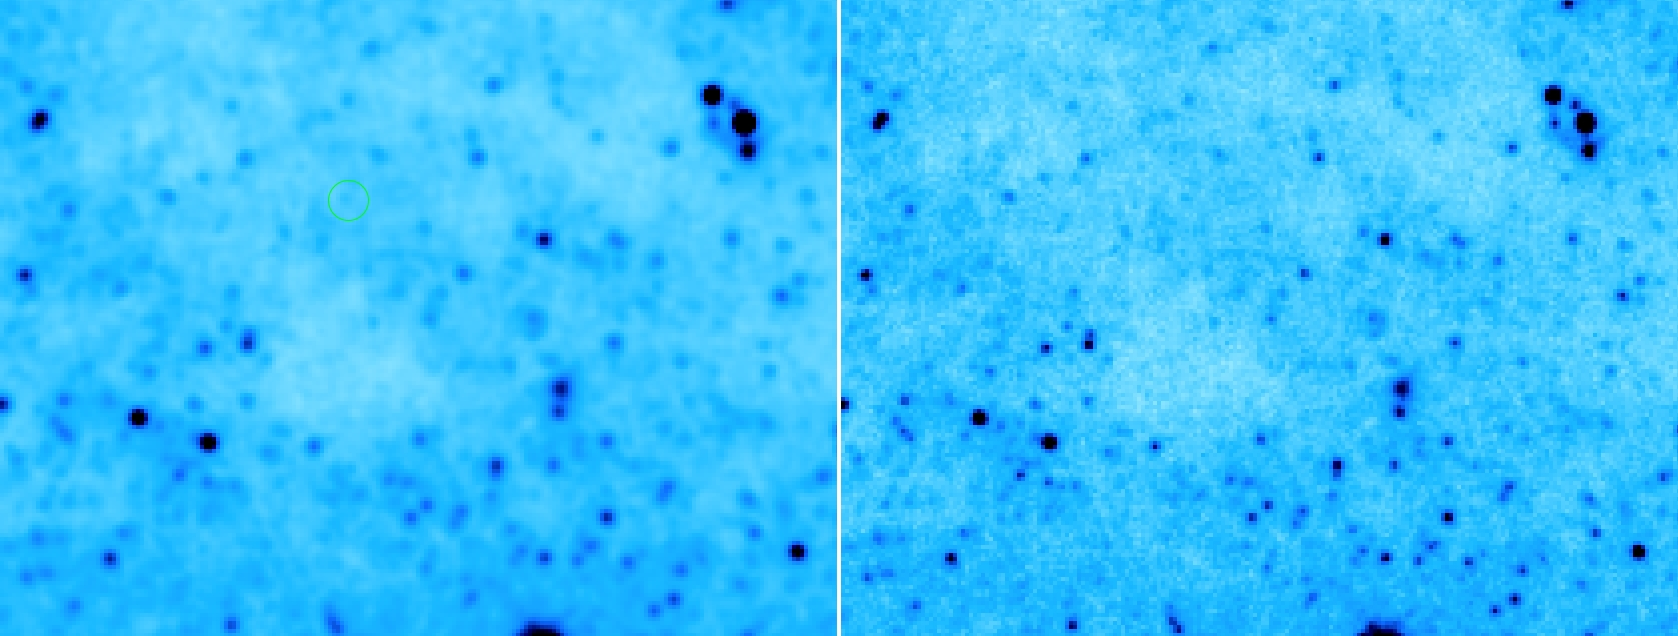
\includegraphics[width=0.87\textwidth]{conv.jpg}
    \caption{In this image you can observe how an observation looks, before and after convolution, this particular image corresponds to the B band filter and was convolved to a 0.083 arcsec FWHM}
    \label{img:conv}
\end{figure}

\begin{table}[h]
  \centering
    \begin{tabular}{ c c c }
    \hline\hline
    
    Filter / Config. & Central $\lambda$ & FWHM (arcsec)\\
    \hline
    
    F225W & 235.9 nm & $\sim$0.083\\
    
    F336W & 335.5 nm & $\sim$0.075\\
    
    F373N & 373.0 nm & $\sim$0.070\\
    
    F438W & 432.5 nm & $\sim$0.070\\
    
    F487N & 487.1 nm & $\sim$0.067\\
    
    F502N & 501.0 nm & $\sim$0.067\\
    
    F657N & 656.7 nm & $\sim$0.070\\
    
    F673N & 676.6 nm & $\sim$0.070\\
    
    F814W & 802.4 nm & $\sim$0.074\\
    
    \hline
  \end{tabular}
  \caption{WFC3/UVIS PSF FWHM informations for the selected dataset, as you can see the largest number here is 0.083 wich means the poorest spatial resolution, this is the number used to calculate the convolution kernel, in order to precess them all images must have the same spatial resolution.}
  \label{tab:dos}
\end{table}

After convoling all the picures, I started to do some tests, but I realized that maybe around 30\% of the images was missing information and/or noise and the results I was getting were mislead by the outliers. In clustering algorithms we must help the algorithm, make sure that what we are inputing is something that can be clustered, although some of them are \emph{shielded} against outliers, making our data more accesible and easy for the neural networks to interpret will help you to get better results, as you can see in image \ref{img:dos} (open one and explore it in DS9) there is missing information and noise. In order to correct this I decided to go with the easiest way I could think of, just cut the image. And I did selected a processable area excluding all the missing information and noisy areas.

\begin{figure}[h]
	\centering
    \includegraphics[width=0.47\textwidth]{uno.jpg}
    \caption{Look at the image, it is composed of two mosaics, therefore, there are some regions with missing data, now look at the borders of each mosaic there is noise near the edges, this is data that we don't want messing with our clustering algorithm and can be classifed as outliers, it is very important to reduce them as much as possbile so the output clusters can be correclty classified and correspond to the information that we are looking for}
    \label{img:dos}
\end{figure}

The next step was to build the datacube, at this point you can decide if you want to process your images indendently or all of them. The ideal here is to input all of them in a datacube, so the output cluters relate information from all the wavelenghts and the regions covered by them can be interpreted more easily. Now if you choose to create an imagecube (just append the image arrays in one FITS file) it is posible that youy images have a different conversion between their world coordinate system to pixel, so have to make sure all of your images are projected with only one conversion, this mean that you have to reproject them to a common WCS.

Well, what I wrote before it is a brief summary of what I did, but I'm sure that you can find a better way to do your own data pre-processing but here are some things that you should consider:
	\begin{itemize}
    	\item Create a methond as general as possible, with input parameter that can be adapted to any kind of data, this will save you a lot of work in the future
        \item Understand first your algorithm, how the data is going to be processed and design the best way to input your data
        \item Accomodate your data according to the type of attributes that the algorithm can handle
        \item Consider the size of your dataset, if it's huge your program may never end
        \item Find out of your algorithm can work with high dimensional data (multi-wavelenght), because if not, you won't be able to input datacubes
        \item Find out if your selected clustering algorithms is able to find clusters of irregular shapes, this will help you to device the best way to accomodate your patterns
        \item Handle outliers, if you identify them, know where they are, try to eliminate them as much as possible, we don't want them messing with our clusters
        \item In case that you come up with an artful mathematical method like PCA to reduce dimensionality, make sure that what you input can later make sense when is clustered, becuase you will be working in another space
        \item Remeber that the most important goal is to find hidden knowledge therefore, you must know you to visualize and interpret your results
        \item For the let's call it \emph{astronomy image processing}, make sure that your data is scientifically aproved ask people around you.
    \end{itemize}

%Convolution
%Cropping
%Repgojection
%Cubbing
%Explain the main rules of why to preprocess the data

This section is explained at lenght in the GitHub page, there you will find my codes and some helpful links, \url{https://github.com/LaurethTeX/Clustering/blob/master/Preprocessing.md}

\section{Software available}
%Como hacer preprocessing en los datos
For doing data preprocessing there are a bunch of softwares available, even there is one being developed by Sophia Lianou called \emph{imagecube} which, when it is finished, will be one of the best, has everything you need in one package. I'll say that this part is yours to discover, everyday there are more and more being released or new versions of the existent ones but in the meanwhile it will depend entirely on you, which software you want to use. For \emph{Python} all the functions you will need can be found in the \emph{Astropy} module, \textbf{check the API!!!.}


This specific part is all explained in GitHub in this link. \url{https://github.com/LaurethTeX/Clustering/blob/master/Preprocessing.md#first-step-data-pre-processing}

\begin{remark}
	Some links to start,
    \begin{itemize}
    	\item Astropy, Convolution and filtering, \url{http://docs.astropy.org/en/stable/convolution/index.html}
        \item AstroDrizzle: New Software for Aligning and Combining
HST Images, With Improved Handling of Astrometric Data, \url{http://drizzlepac.stsci.edu/}
		\item Tiny Tim HST PSF Modeling, \url{http://www.stsci.edu/hst/observatory/focus/TinyTim}
        \item IRAF, Image Reduction and Analysis Facility, \url{http://iraf.noao.edu/}
    \end{itemize}
\end{remark}

\chapterimage{ddd.jpg} % Chapter heading image

\chapter{Istoria Antică. Roma}
\epigraph{Corrige praetertum, praesens rege, cerne futurum - Analizeaza trecutul, conducete de prezent, prevede viitorul }{Lucius Annaeus Seneca minor}
\section{Ce este istoria ?}\index{Ce este istoria ?}

Interesul faţă de trecut este specific rasei umane. Acest interes este greu de explicat doar prin o curiozitate umană. Faptul că omul însuşi  este o fiinţă istorică.  El se dezvoltă şi să schimbă în timp, fiind produsul a acestei dezvoltări.

Sensul originar al cuvântului "istorie" vine din vechea  greacă  ce insemna "anchetă", "recunoaştere", "înfiinţarea". În antichitate cuvântului "istoria" era folosit ca determinarea cunoştinţelor obţinute prin cercetări în general, adică nu numai despre evenimentele din trecut cum suntem deprişi să folosim acest cuvînt astăzi. Astfel, Aristotel a folosit acest cuvînt în "Istoria animalelor". De asemenea, îl găsim în imnurile lui Homer, scrierile lui Heraclit şi în textul jurîmântului statului atenian.



În mitologia greacă, patronatul asupra istoriei era asigurat de una din muze Clio - o femeie tânără, cu o faţă înspirată, cu un papirus sau pergament în mînă. Numele  muzei Clio - este o derivată  a cuvîntului  grecesc "laudă".



\section{Istoria ca ştiinţă}\index{Istoria ca ştiinţă}
\epigraph{Historia est Magistra Vitae}{Marcus Tullius Cicero}
After I arrived and had my first meeting with Pauline, she explained me a general idea of what she wanted and shared me some more papers (about multi-wavelenght studies), I read the information and came up with the objective.

\begin{itemize}
\item Find out a method to transform data from a high dimensional dataset (FITS cube or any other data arrangement) to a low dimensional understandable information (graphs, clusters).
\end{itemize}

This means that from multiple images with different wavelengths of the same target apply an algorithm to find the hidden patterns that lie hidden between them.

\section{Ştiinţele istorice}\index{Ştiinţele istorice}
Ok, here is where I explain from where this is going to start, at that time I just had a microcontrollers and engineering design course my mind was set completelly to find appplicable theories and create uselful things with them, which is the complete opposite of how astronomy works. First, there's no way to test an experiment with galaxies and most of the information is fuzzy and subjective (not all). The process of having an, let's say \emph{astronomy idea} is a result of applying all your physics knowledge and consider the \textbf{cosmological principle},
\begin{quote}
The (testable) assumption that the same physical laws that apply here and now also apply everywhere and at all times, and that there are no special locations or directions in the universe.
\end{quote}

That's how science is made, thinking and testing and thinking again, creating your own scientific method, comming up with hypothesis, learning what might work and what not, using your insticts. 

Well, before comming here I didn't think like that, it was just all about being super productive and thinking about doing robots and all kinds of devices with sensors. I had some experience programming in C/C++, no computer science backgound and I had never had an astronomy course.

This report was written in order to help someone to continue researching about data mining techniques applied in Astronomy, I explain how did I come up with the clustering techniques, my hypothesis, some tests and other ideas I have had, I hope this can help anyone and the research is continued. Anything you may need/questions do not hesitate to contact me, my e-mail address is: \emph{mrs.petzl@gmail.com}, also s part of my own documentation I created a GitHub page where you can download all the codes I programmed and find more information. The link to this page is: \url{https://github.com/LaurethTeX/Clustering}, from the \textsc{readme} file you can acces to all the pages, take your time to surf.
%------------------------------------------------

\subsection{References}\index{References}

Since I found so much good information about pretty much everything I wanted to know about, I will just create a remark and let you know where you can find more specific information about, just like below.

\begin{remark}
For more information about the cosmological principle, review Chapter 1: Why Learn Astronomy?, page 10, from \textbf{21st Century Astronomy}, \textit{Hester | Smith | Blumenthal | Kay | Voss}, Third Edition, 2010.
\end{remark}
\begin{expli}
For more information about the cosmological principle, review Chapter 1: Why Learn Astronomy?, page 10, from \textbf{21st Century Astronomy}, \textit{Hester | Smith | Blumenthal | Kay | Voss}, Third Edition, 2010.
\end{expli}


%This statement requires citation \cite{book_key}; this one is more specific \cite[122]{article_key}.

\chapterimage{ddd.jpg} % Chapter heading image

\chapter{Istoria Medievală AUUUU}
\epigraph{Corrige praetertum, praesens rege, cerne futurum - Analizeaza trecutul, conducete de prezent, prevede viitorul }{Lucius Annaeus Seneca minor}
\section{Ce este istoria ?}\index{Ce este istoria ?}

Interesul faţă de trecut este specific rasei umane. Acest interes este greu de explicat doar prin o curiozitate umană. Faptul că omul însuşi  este o fiinţă istorică.  El se dezvoltă şi să schimbă în timp, fiind produsul a acestei dezvoltări.

Sensul originar al cuvântului "istorie" vine din vechea  greacă  ce insemna "anchetă", "recunoaştere", "înfiinţarea". În antichitate cuvântului "istoria" era folosit ca determinarea cunoştinţelor obţinute prin cercetări în general, adică nu numai despre evenimentele din trecut cum suntem deprişi să folosim acest cuvînt astăzi. Astfel, Aristotel a folosit acest cuvînt în "Istoria animalelor". De asemenea, îl găsim în imnurile lui Homer, scrierile lui Heraclit şi în textul jurîmântului statului atenian.



În mitologia greacă, patronatul asupra istoriei era asigurat de una din muze Clio- o femeie tânără, cu o faţă înspirată, cu un papirus sau pergament în mînă. Numele  muzei Clio - este o derivată  a cuvîntului  grecesc "laudă".



\section{Istoria ca ştiinţă}\index{Istoria ca ştiinţă}
\epigraph{Historia est Magistra Vitae}{Marcus Tullius Cicero}
After I arrived and had my first meeting with Pauline, she explained me a general idea of what she wanted and shared me some more papers (about multi-wavelenght studies), I read the information and came up with the objective.

\begin{itemize}
\item Find out a method to transform data from a high dimensional dataset (FITS cube or any other data arrangement) to a low dimensional understandable information (graphs, clusters).
\end{itemize}

This means that from multiple images with different wavelengths of the same target apply an algorithm to find the hidden patterns that lie hidden between them.

\section{Ştiinţele istorice}\index{Ştiinţele istorice}
Ok, here is where I explain from where this is going to start, at that time I just had a microcontrollers and engineering design course my mind was set completelly to find appplicable theories and create uselful things with them, which is the complete opposite of how astronomy works. First, there's no way to test an experiment with galaxies and most of the information is fuzzy and subjective (not all). The process of having an, let's say \emph{astronomy idea} is a result of applying all your physics knowledge and consider the \textbf{cosmological principle},
\begin{quote}
The (testable) assumption that the same physical laws that apply here and now also apply everywhere and at all times, and that there are no special locations or directions in the universe.
\end{quote}

That's how science is made, thinking and testing and thinking again, creating your own scientific method, comming up with hypothesis, learning what might work and what not, using your insticts. 

Well, before comming here I didn't think like that, it was just all about being super productive and thinking about doing robots and all kinds of devices with sensors. I had some experience programming in C/C++, no computer science backgound and I had never had an astronomy course.

This report was written in order to help someone to continue researching about data mining techniques applied in Astronomy, I explain how did I come up with the clustering techniques, my hypothesis, some tests and other ideas I have had, I hope this can help anyone and the research is continued. Anything you may need/questions do not hesitate to contact me, my e-mail address is: \emph{mrs.petzl@gmail.com}, also s part of my own documentation I created a GitHub page where you can download all the codes I programmed and find more information. The link to this page is: \url{https://github.com/LaurethTeX/Clustering}, from the \textsc{readme} file you can acces to all the pages, take your time to surf.
%------------------------------------------------

\subsection{References}\index{References}

Since I found so much good information about pretty much everything I wanted to know about, I will just create a remark and let you know where you can find more specific information about, just like below.

\begin{remark}
For more information about the cosmological principle, review Chapter 1: Why Learn Astronomy?, page 10, from \textbf{21st Century Astronomy}, \textit{Hester | Smith | Blumenthal | Kay | Voss}, Third Edition, 2010.
\end{remark}
\begin{expli}
For more information about the cosmological principle, review Chapter 1: Why Learn Astronomy?, page 10, from \textbf{21st Century Astronomy}, \textit{Hester | Smith | Blumenthal | Kay | Voss}, Third Edition, 2010.
\end{expli}


%This statement requires citation \cite{book_key}; this one is more specific \cite[122]{article_key}.

\chapterimage{ddd.jpg} % Chapter heading image

\chapter{Istoria Medievală este}
\epigraph{Corrige praetertum, praesens rege, cerne futurum - Analizeaza trecutul, conducete de prezent, prevede viitorul }{Lucius Annaeus Seneca minor}
\section{Ce este istoria ?}\index{Ce este istoria ?}

Interesul faţă de trecut este specific rasei umane. Acest interes este greu de explicat doar prin o curiozitate umană. Faptul că omul însuşi  este o fiinţă istorică.  El se dezvoltă şi să schimbă în timp, fiind produsul a acestei dezvoltări.

Sensul originar al cuvântului "istorie" vine din vechea  greacă  ce insemna "anchetă", "recunoaştere", "înfiinţarea". În antichitate cuvântului "istoria" era folosit ca determinarea cunoştinţelor obţinute prin cercetări în general, adică nu numai despre evenimentele din trecut cum suntem deprişi să folosim acest cuvînt astăzi. Astfel, Aristotel a folosit acest cuvînt în "Istoria animalelor". De asemenea, îl găsim în imnurile lui Homer, scrierile lui Heraclit şi în textul jurîmântului statului atenian.



În mitologia greacă, patronatul asupra istoriei era asigurat de una din muze Clio- o femeie tânără, cu o faţă înspirată, cu un papirus sau pergament în mînă. Numele  muzei Clio - este o derivată  a cuvîntului  grecesc "laudă".



\section{Istoria ca ştiinţă}\index{Istoria ca ştiinţă}
\epigraph{Historia est Magistra Vitae}{Marcus Tullius Cicero}
After I arrived and had my first meeting with Pauline, she explained me a general idea of what she wanted and shared me some more papers (about multi-wavelenght studies), I read the information and came up with the objective.

\begin{itemize}
\item Find out a method to transform data from a high dimensional dataset (FITS cube or any other data arrangement) to a low dimensional understandable information (graphs, clusters).
\end{itemize}

This means that from multiple images with different wavelengths of the same target apply an algorithm to find the hidden patterns that lie hidden between them.

\section{Ştiinţele istorice}\index{Ştiinţele istorice}
Ok, here is where I explain from where this is going to start, at that time I just had a microcontrollers and engineering design course my mind was set completelly to find appplicable theories and create uselful things with them, which is the complete opposite of how astronomy works. First, there's no way to test an experiment with galaxies and most of the information is fuzzy and subjective (not all). The process of having an, let's say \emph{astronomy idea} is a result of applying all your physics knowledge and consider the \textbf{cosmological principle},
\begin{quote}
The (testable) assumption that the same physical laws that apply here and now also apply everywhere and at all times, and that there are no special locations or directions in the universe.
\end{quote}

That's how science is made, thinking and testing and thinking again, creating your own scientific method, comming up with hypothesis, learning what might work and what not, using your insticts. 

Well, before comming here I didn't think like that, it was just all about being super productive and thinking about doing robots and all kinds of devices with sensors. I had some experience programming in C/C++, no computer science backgound and I had never had an astronomy course.

This report was written in order to help someone to continue researching about data mining techniques applied in Astronomy, I explain how did I come up with the clustering techniques, my hypothesis, some tests and other ideas I have had, I hope this can help anyone and the research is continued. Anything you may need/questions do not hesitate to contact me, my e-mail address is: \emph{mrs.petzl@gmail.com}, also s part of my own documentation I created a GitHub page where you can download all the codes I programmed and find more information. The link to this page is: \url{https://github.com/LaurethTeX/Clustering}, from the \textsc{readme} file you can acces to all the pages, take your time to surf.
%------------------------------------------------

\subsection{References}\index{References}

Since I found so much good information about pretty much everything I wanted to know about, I will just create a remark and let you know where you can find more specific information about, just like below.

\begin{remark}
For more information about the cosmological principle, review Chapter 1: Why Learn Astronomy?, page 10, from \textbf{21st Century Astronomy}, \textit{Hester | Smith | Blumenthal | Kay | Voss}, Third Edition, 2010.
\end{remark}
\begin{expli}
For more information about the cosmological principle, review Chapter 1: Why Learn Astronomy?, page 10, from \textbf{21st Century Astronomy}, \textit{Hester | Smith | Blumenthal | Kay | Voss}, Third Edition, 2010.
\end{expli}


%This statement requires citation \cite{book_key}; this one is more specific \cite[122]{article_key}.




%----------------------------------------------------------------------------------------
%	CHAPTER 3
%----------------------------------------------------------------------------------------

\chapterimage{boat.png}
\chapter{Understand your data}

Before continuing, first and most importantly you must select the \emph{raw} data you are going to process and later after you aquire experience with an specific dataset the idea is to expand the algorithms to any kind of dataset. The important things are to learn how to input the data correctly, establish the right \emph{learning paramenters} in the selected algorithm and find the best way to visualize your results and interpret them correctly.

Now let's start with basic concepts that vary from an engineering to an astronomer point of view.
\section{What is an image?}
	As you may know, an image is a matrix of numbers that cointains the specific brightness level that corresponds to a given pixel. And from there the concepts evolves and adds channels of colour and depth. But for now, let's just think about monochromatic images (only one channel). In Astronomy, images are usually considered sets of scientific data, observations, that contain information about an speficic target in the sky seen throught an specific filter and the levels of brightness correspond to the behaviour of the optical sensor (CCD camera) in relation with the number of electrons that hit a particular pixel through an specific waveband. Something else to consider is that the sky is not flat with this I mean that the celestial vault is like a sphere surrounding us therefore cartesian coorditanes are not the paramenters used to identify points in space, there is another system called WCS (World Coordinate System) hence a conversion between pixels and WCS coordinates exists. As you are realizing now just one image can contain tons of information related to it, now imagine that multiplied for terabytes and terabytes of stars, galaxies, planets, nebulae or any object in space. Fortunately in astronomy this is solved using an image format that cointains the image and its own information.
	\subsection{FITS files}
    	This format is the standard data format used in astronomy, can contain one image, multiple images, tables and header keywords providing descriptive information about the data. The way it works is that this format can contain a text file with keywords that comprise the information about the observation and a multidimensional array that could be a table, or an image, or an array of images (data cube). This files can be managed in diffetent ways, with an image preview use DS9, for handing the data in a program use the \emph{Python} package \emph{PyFITS}.
        
	\subsection{WFC3 ERS M83 Data Products}
    The selected dataset to test the data mining libraries I found is a series of observations of M83 at 9 different wavelengths, the original images can be found in this webpage, \url{http://archive.stsci.edu/prepds/wfc3ers/m83datalist.html}, the specific information about them can be found in Table \ref{tab:uno}. This particular images were observed through HST with the WFC3/UVIS camera.
    
\begin{table}[h]
  \centering
  \begin{tabular}{ c c c c c c }
    \hline\hline
    Filter / Config. & Waveband / Central $\lambda$/ Line & Obs. Date & Comment \\
    \hline
    F225W & UV filter / 235.9 nm & 26 Aug 2009 &  UV wide\\
    
    F336W & UV filter / 335.5 nm & 26 Aug 2009 & Str$\ddot{o}$mgren $u$\\
    
    F373N & Narrow-Band Filter / 373.0 nm & 19 Aug 2009 & Includes \textsc{[OII]}\\
    
    F438W & Wide-Band Filter / 432.5 nm & 26 Aug 2009 & $B$, Johnson-Cousins set\\
    
    F487N & Narrow-Band Filter / 487.1 nm & 25 Aug 2009 & Includes H$\beta$\\
    
    F502N & Narrow-Band Filter / 501.0 nm & 26 Aug 2009 & Includes \textsc{[O III]}\\
    
    F657N & Narrow-Band Filter / 656.7 nm & 25 Aug 2009 & Includes H$\alpha$+\textsc{[NII]}\\
    
    F673N & Narrow-Band Filter / 676.6 nm & 20 Aug 2009 & Includes \textsc{[SII]}\\
    
    F814W & Wide-Band Filter / 802.4 nm & 26 Aug 2009 & $I$, Johnson-Cousins set\\
    \hline
  \end{tabular}
  \caption{Summary of Observations}
  \label{tab:uno}
\end{table}
%Poner aqui la tabla con los datos de acada filtro
%No olvidar poner en GitHub el programa de como hacer el cube y tammbien el de reproject cube con montrage wrapper

\section{Preprocessing your data}
This section is where you prepare your data to be processed, you have to make sure that all your images have the same grid size, same spatial resolution, less possible quantity of outliers abd noise and same coordinate system. Now, what are those things? Same grid size means that your images must have the same pixel size, in the dataset we are processing we don't have to worry about this, the pixel size is 0.0396 arcsec/pixel. Now, spatial resoultion, each image has it's own spatial resolution depending on the filter that was used to get the observation, the number that you will be looking for is the FWHM that describes the PSF of every image. When you have all the FWHM for all the images you should choose the largest which corresponds to the poorest spatial resolution and create a convolution kernel with \emph{Tiny Tim} or use a gaussian kernel calculated with \emph{Astropy} and convolve all the images with that kernel. This exactly what I did, if you look at image \ref{img:conv}, you will see the before and after convolution. In table \ref{tab:dos} you can see how I chose the number for the FWHM.

\begin{figure}[h]
	\centering
    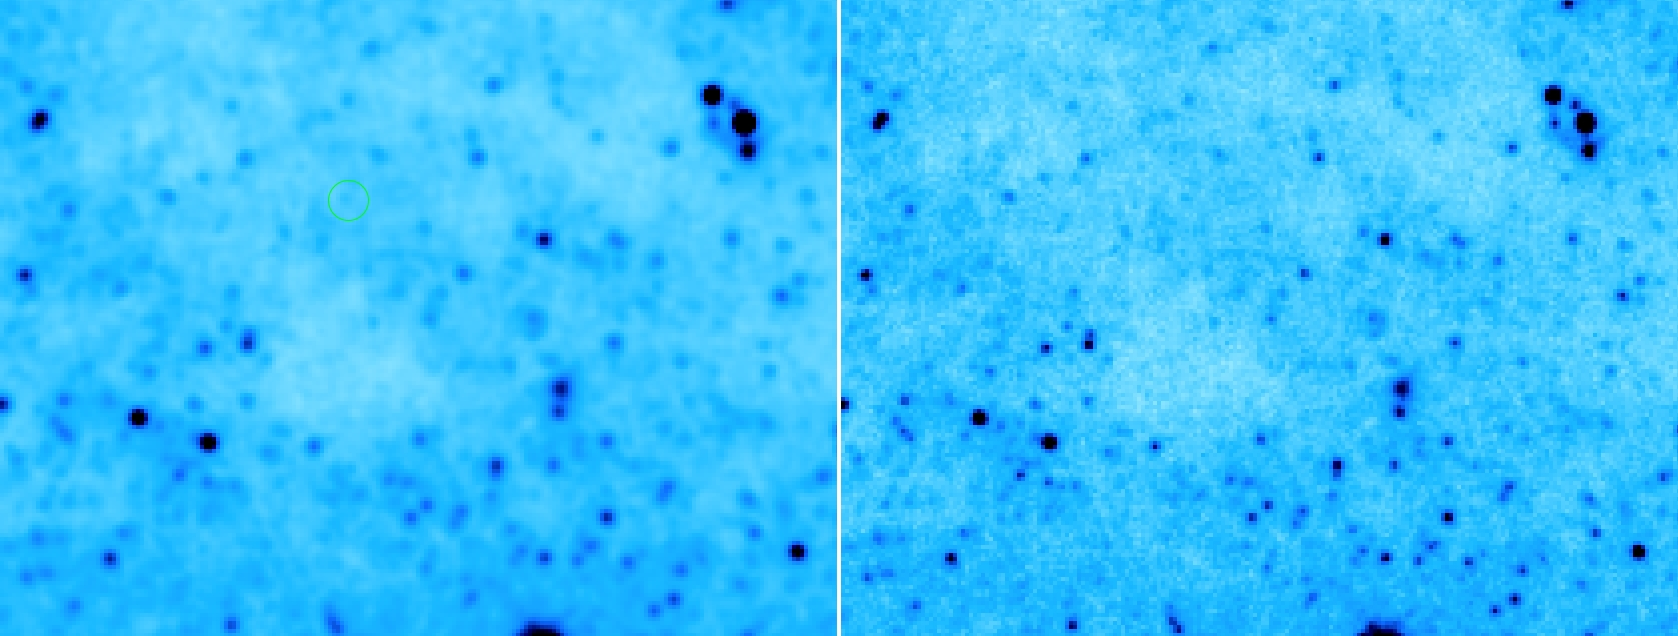
\includegraphics[width=0.87\textwidth]{conv.jpg}
    \caption{In this image you can observe how an observation looks, before and after convolution, this particular image corresponds to the B band filter and was convolved to a 0.083 arcsec FWHM}
    \label{img:conv}
\end{figure}

\begin{table}[h]
  \centering
    \begin{tabular}{ c c c }
    \hline\hline
    
    Filter / Config. & Central $\lambda$ & FWHM (arcsec)\\
    \hline
    
    F225W & 235.9 nm & $\sim$0.083\\
    
    F336W & 335.5 nm & $\sim$0.075\\
    
    F373N & 373.0 nm & $\sim$0.070\\
    
    F438W & 432.5 nm & $\sim$0.070\\
    
    F487N & 487.1 nm & $\sim$0.067\\
    
    F502N & 501.0 nm & $\sim$0.067\\
    
    F657N & 656.7 nm & $\sim$0.070\\
    
    F673N & 676.6 nm & $\sim$0.070\\
    
    F814W & 802.4 nm & $\sim$0.074\\
    
    \hline
  \end{tabular}
  \caption{WFC3/UVIS PSF FWHM informations for the selected dataset, as you can see the largest number here is 0.083 wich means the poorest spatial resolution, this is the number used to calculate the convolution kernel, in order to precess them all images must have the same spatial resolution.}
  \label{tab:dos}
\end{table}

After convoling all the picures, I started to do some tests, but I realized that maybe around 30\% of the images was missing information and/or noise and the results I was getting were mislead by the outliers. In clustering algorithms we must help the algorithm, make sure that what we are inputing is something that can be clustered, although some of them are \emph{shielded} against outliers, making our data more accesible and easy for the neural networks to interpret will help you to get better results, as you can see in image \ref{img:dos} (open one and explore it in DS9) there is missing information and noise. In order to correct this I decided to go with the easiest way I could think of, just cut the image. And I did selected a processable area excluding all the missing information and noisy areas.

\begin{figure}[h]
	\centering
    \includegraphics[width=0.47\textwidth]{uno.jpg}
    \caption{Look at the image, it is composed of two mosaics, therefore, there are some regions with missing data, now look at the borders of each mosaic there is noise near the edges, this is data that we don't want messing with our clustering algorithm and can be classifed as outliers, it is very important to reduce them as much as possbile so the output clusters can be correclty classified and correspond to the information that we are looking for}
    \label{img:dos}
\end{figure}

The next step was to build the datacube, at this point you can decide if you want to process your images indendently or all of them. The ideal here is to input all of them in a datacube, so the output cluters relate information from all the wavelenghts and the regions covered by them can be interpreted more easily. Now if you choose to create an imagecube (just append the image arrays in one FITS file) it is posible that youy images have a different conversion between their world coordinate system to pixel, so have to make sure all of your images are projected with only one conversion, this mean that you have to reproject them to a common WCS.

Well, what I wrote before it is a brief summary of what I did, but I'm sure that you can find a better way to do your own data pre-processing but here are some things that you should consider:
	\begin{itemize}
    	\item Create a methond as general as possible, with input parameter that can be adapted to any kind of data, this will save you a lot of work in the future
        \item Understand first your algorithm, how the data is going to be processed and design the best way to input your data
        \item Accomodate your data according to the type of attributes that the algorithm can handle
        \item Consider the size of your dataset, if it's huge your program may never end
        \item Find out of your algorithm can work with high dimensional data (multi-wavelenght), because if not, you won't be able to input datacubes
        \item Find out if your selected clustering algorithms is able to find clusters of irregular shapes, this will help you to device the best way to accomodate your patterns
        \item Handle outliers, if you identify them, know where they are, try to eliminate them as much as possible, we don't want them messing with our clusters
        \item In case that you come up with an artful mathematical method like PCA to reduce dimensionality, make sure that what you input can later make sense when is clustered, becuase you will be working in another space
        \item Remeber that the most important goal is to find hidden knowledge therefore, you must know you to visualize and interpret your results
        \item For the let's call it \emph{astronomy image processing}, make sure that your data is scientifically aproved ask people around you.
    \end{itemize}

%Convolution
%Cropping
%Repgojection
%Cubbing
%Explain the main rules of why to preprocess the data

This section is explained at lenght in the GitHub page, there you will find my codes and some helpful links, \url{https://github.com/LaurethTeX/Clustering/blob/master/Preprocessing.md}

\section{Software available}
%Como hacer preprocessing en los datos
For doing data preprocessing there are a bunch of softwares available, even there is one being developed by Sophia Lianou called \emph{imagecube} which, when it is finished, will be one of the best, has everything you need in one package. I'll say that this part is yours to discover, everyday there are more and more being released or new versions of the existent ones but in the meanwhile it will depend entirely on you, which software you want to use. For \emph{Python} all the functions you will need can be found in the \emph{Astropy} module, \textbf{check the API!!!.}


This specific part is all explained in GitHub in this link. \url{https://github.com/LaurethTeX/Clustering/blob/master/Preprocessing.md#first-step-data-pre-processing}

\begin{remark}
	Some links to start,
    \begin{itemize}
    	\item Astropy, Convolution and filtering, \url{http://docs.astropy.org/en/stable/convolution/index.html}
        \item AstroDrizzle: New Software for Aligning and Combining
HST Images, With Improved Handling of Astrometric Data, \url{http://drizzlepac.stsci.edu/}
		\item Tiny Tim HST PSF Modeling, \url{http://www.stsci.edu/hst/observatory/focus/TinyTim}
        \item IRAF, Image Reduction and Analysis Facility, \url{http://iraf.noao.edu/}
    \end{itemize}
\end{remark}


%----------------------------------------------------------------------------------------
%	CHAPTER 4
%----------------------------------------------------------------------------------------

\chapterimage{head1.png} % Chapter heading image

\chapter{Experimenting}

I discovered surfing on the internet a cloud computing software that is free, has data mining algorithms embeded, is specifically developed for Astronomy and is programmed by Caltech, University Federico II and the Astronomical Observatory of Capodimonte. The homepage website, \url{http://dame.dsf.unina.it/index.html}. Well, the platform for testing is ready!, now what? I requested and account and the next day they sent me an acceptance with my username and my password approved.
I introduced myself to the documentation, the available clustering funcionts, the manuals for every method, the blogs and discovered that the was one method available that could work with datacubes and do its clustering on every pattern (number in the multidimensional matrix) which was exaclty what I needed. The name of this method is ESOM (Evolving Self Organizing Maps) and I read its manual, did some foolish test with all my image and ... never got a result ... the experiment ran forever (more than two weeks), when I realised that this wasn't the best way to tackle this problem I started considering only clustering on the independent images and not in the datacube due to the fact that the dimensionality was inmense. So, in the end my selected methods have some results but not all, here is where all the work has to be done, analyzed and tested again.

\section{Methods Selected}

\subsection{ESOM, Evolving Self Organizing Maps}
The \emph{official} manual for this method can de found here, \url{http://dame.dsf.unina.it/documents/ESOM_UserManual_DAME-MAN-NA-0021-Rel1.2.pdf}, there you will find a full explanation of the method, the meaning of every variable and the supported file types.

Here is my own explanation of how this particular method works, first of all, can be used as an unsupervised machine learning technique or you can help the algorithm to identify regions an make it a supervised machine learnig technique, this type of clustering finds groups of patterns with similarities and preserves its topology, starts with a null network without any nodes and those are creted incrementally when a new input pattern is presented, the prototype nodes in the network compete with each other and the connections of the winner node are updated. 

The method is divided in three stages, \emph{Train}, \emph{Test} and \emph{Run}.
The first step to experiment with this method is Train. Here, the important variables to undertand an look at are, the learning rate, epsilon and the pruning frequency. It is highly recomendable that you check the DAMEWARE manual for this function, there they will explain in detail the meaning of each on the mentioned variables.
% fULL AND SAMPLE DATACUBE
\subsubsection{Expected Results}
	This particular method as I mentioned before supports datacubes and considers as an independent pattern all the  numbers in the multi-dimensional array this means that our clusters are groups of patterns with similar characteristics, that correspond to volumes of similar fluxes of electrons inside the datacube.
    
    The output files from the experiment that will show us our results are, 
    \begin{itemize}
    	\item \emph{E\_SOM\_Train\/Test\/Run\_Results.txt}: File that, for each pattern, 
reports ID, features, BMU, cluster and activation of winner node
		\item \emph{E\_SOM\_Train\/Test\/Run\_Histogram.png}: Histogram of clusters found 
        \item \emph{E\_SOM\_Train\/Test\/Run\_U\_matrix.png}: U-Matrix image 
        \item \emph{E\_SOM\_Train\/Test\/Run\_Clusters.txt}: File that, for each clusters, reports label, number of pattern assigned, percentage of association respect total number of pattern and its centroids. 
        \item \emph{E\_SOM\_Train\_Datacube\_image.zip}: Archive that includes the 
clustered images of each slice of a datacube.\footnote{I have my doubts whether this file is produced or not, in none of my test was produced, you might need to contact the developers and ask about this.}
    \end{itemize}
The file that you will be looking forward to see is the last one, the zip where you will be able to see the slices of the volume, and how the final configuration of the clusters was arranged.

\subsubsection{Failed and still running tests: What no to do and what is still running}
The first tests I did included all the complete datacube, including the areas where data was missing, the images were only reprojected and convolved. That was before realising that outliers migth affect the ability of the algorithm to identify the clusters and distract them with noise and missing data. So, the first thing you must NOT do, is to get rid of the outliers when you are training your network, if you ever get to have a well trained network then it might be interesting to learn how the network interacts with noise an outliers, but for now we will help her a bit. 

In table \ref{tab:ds9failed} are the input parameters I used to the failed tests applied in the \emph{raw} datacube, and in table \ref{tab:ds9running} are the input parameters used on experimets that are stil running since August 7th, 2014. (I wonder if they will ever end)

\begin{table}[h!]
  \centering
    \begin{tabular}{ c c c c c c }
    \hline\hline
    
    Name & Input nodes & Normalized data & Learning rate & Epsilon & Pruning Frequency\\
    \hline
    
    Train2 & 1 & 1 & 0.3 & 0.001 & 5\\
    Train3 & 1 & 1 & 0.7 & 10 & 100\\
    Train4 & 1 & 1 & 0.95 & 1 & 10\\
    Train5 & 1 & 1 & 0.99 & 0.1 & 10\\
    Train6 & 1 & 1 & 0.01 & 0.01 & 1\\
    Train7 & 1 & 1 & 0.5 & 0.7 & 5\\
    Train8 & 1 & 1 & 0.5 & 0.5 & 7\\
    Train11 & 1 & 1 & 0.25 & 0.00001 & 10\\
    
    \hline
  \end{tabular}
  \caption{This table describes all the failed experiments done in the workspace WFC3 with the \emph{raw} datacube as an input, using the ESOM method in the DAME platform selecting the number 3 as the dataset type and without using a previous configuration file.}
  \label{tab:ds9failed}
\end{table}

\begin{table}[h!]
  \centering
    \begin{tabular}{ c c c c c c }
    \hline\hline
    
    Name & Input nodes & Normalized data & Learning rate & Epsilon & Pruning Frequency\\
    \hline
    
    Train9 & 1 & 1 & 0.3 & 0.0001 & 5\\
    Train10 & 1 & 1 & 0.99 & 0.0001 & 10\\
    Train12 & 1 & 1 & 0.5 & 0.0001 & 5\\
    
    \hline
  \end{tabular}
  \caption{This table describes all the experiments done in the workspace WFC3 that are still running since August 7th, 2014 with the \emph{raw} datacube as an input, using the ESOM method in the DAME platform selecting the number 3 as the dataset type and without using a previous configuration file.}
  \label{tab:ds9running}
\end{table}

Some of the failed experiments had histogram like the one you can see on figure \ref{img:faildtrain2} where the cluters were created but reached a point where the neural network could not define how to differenciate a cluster from another clusted and failed.

\begin{figure}[h!]
	\centering
    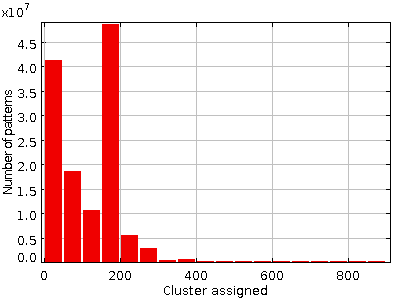
\includegraphics[width=0.47\textwidth]{Histogram_train2.png}
    \caption{In this particular experiment, the neural network failed due to a very low prunning frequency, high number of patterns and all the outliers inclusions.}
    \label{img:faildtrain2}
\end{figure}

Hey, if you were wondering why I always choose to normilize, and one as the input node, well the normalization is due to the fact that I know that the data has, according to its filter, all kinds of ranges of fluxes on every layer which means that the distances between patterns might not be correct, this is a topic you should look into. And for the input node I choose 1 because if I start with any other number the experiment automatically fails, and of course we do not want that.

As I progressed and saw the results and the \emph{log files} in all the failed experiments I decide to try the algorithm on independent layers and see if I could get something. Therefore I selected the H$\alpha$ convolved observation (halpha\_conv.fits) and did some tests on it, table \ref{tab:hafailed} shows the parameters I used for the failed experiments and table \ref{tab:harun} shows the paramters fo the still running experiments.

\begin{table}[h!]
  \centering
    \begin{tabular}{ c c c c c c }
    \hline\hline
    
    Name & Input nodes & Normalized data & Learning rate & Epsilon & Pruning Frequency\\
    \hline
    
    TrainHa1 & 1 & 1 & 0.5 & 0.01 & 5\\
    TrainHa2 & 1 & 1 & 0.5 & 0.001 & 5\\
    
    \hline
  \end{tabular}
  \caption{This table describes the failed experiments done in the workspace WFC3 for the \emph{halpha\_conv.fits} file, using the ESOM method for one layer in the DAME platform selecting the number 3 as the dataset type and without using a previous configuration file.}
  \label{tab:hafailed}
\end{table}

\begin{table}[h!]
  \centering
    \begin{tabular}{ c c c c c c }
    \hline\hline
    
    Name & Input nodes & Normalized data & Learning rate & Epsilon & Pruning Frequency\\
    \hline
    
    TrainHa3 & 1 & 1 & 0.5 & 0.0001 & 5\\
    
    \hline
  \end{tabular}
  \caption{This table describes the still running experiments since August 10th, 2014 in the workspace WFC3 for the \emph{halpha\_conv.fits} file, using the ESOM method for one layer in the DAME platform selecting the number 3 as the dataset type and without using a previous configuration file.}
  \label{tab:harun}
\end{table}

My next mental step was to repeat the tests eliminating as many outliers I could reduce, my hypothesis here is that, if I elimante all the areas where there is missing data and noise, the neural networks will be concentrated only in the patterns I'm interested in clustering and maybe idenfying interesting regions that correspond to some known interstellar object. So, what I did was to try the ESOM algorithm with, again, independent images, this time I decided to apply the same experiment to three different layers, H$\alpha$, UV wide and $i$-band. In table \ref{tab:threefail} you can see the parameters of the failed experiments and on figure \ref{img:fail3} there are some of the output histograms. Also, in table \ref{tab:threerun} you can see the input parameters of the still running experiments.

\begin{table}[h!]
  \centering
    \begin{tabular}{ c c c c c c }
    \hline\hline
    
    Name & Input nodes & Normalized data & Learning rate & Epsilon & Pruning Frequency\\
    \hline
    
    Train1 & 1 & 1 & 0.5 & 0.001 & 50\\
    Train2 & 1 & 1 & 0.5 & 0.01 & 50\\
    Train3 & 1 & 1 & 0.5 & 0.1 & 100\\
    Train4 & 1 & 1 & 0.5 & 0.001 & 100\\
    
    \hline
  \end{tabular}
  \caption{This parametes where used in three different workspaces (\emph{halphaCrop, uvwidecrop, ibandcrop}), with their own input file that corresponded to the convolved and cropped observation of each filter (halpha\_conv\_crp.fits, uvwide\_conv\_crp.fits, iband\_conv\_crp.fits), all of the experiments had no previous configuration file and the dataset type was 3 and all failed.}
  \label{tab:threefail}
\end{table}

\begin{figure}[h!]
	\centering
    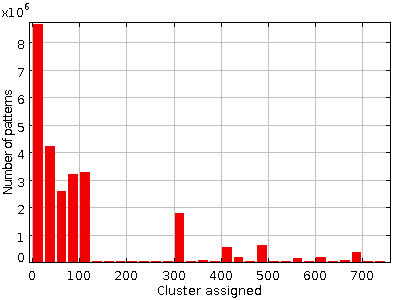
\includegraphics[width=0.31\textwidth]{Histogram-halpha1.png}
    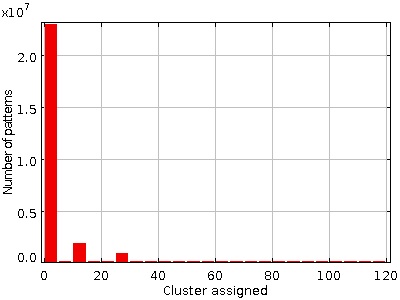
\includegraphics[width=0.31\textwidth]{Histogram-uvwide-2.png}
    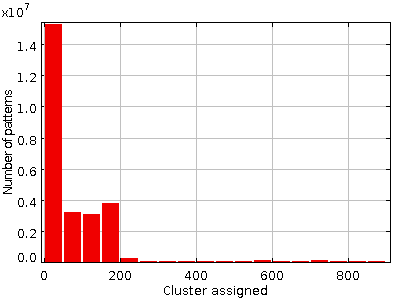
\includegraphics[width=0.31\textwidth]{Histogram-iband3.png}
    \caption{The histogram on the left corresponds to the halpha workspace in Train1, the one on the center to the iband workspace in Train3 and the one on the right to the uvwide workspace in Train2, all of them were failed experiments.}
    \label{img:fail3}
\end{figure}

\begin{table}[h!]
  \centering
    \begin{tabular}{ c c c c c c }
    \hline\hline
    
    Name & Input nodes & Normalized data & Learning rate & Epsilon & Pruning Frequency\\
    \hline
    
    Train5 & 1 & 1 & 0.5 & 0.0001 & 100\\
    Train6 & 1 & 1 & 0.99 & 0.0001 & 75\\

    \hline
  \end{tabular}
  \caption{This parametes where used in three different workspaces (\emph{halphaCrop, uvwidecrop, ibandcrop}), with their own input file that corresponded to the convolved and cropped observation of each filter (halpha\_conv\_crp.fits, uvwide\_conv\_crp.fits, iband\_conv\_crp.fits), all of the experiments had no previous configuration file and the dataset type was 3. The experiments mentioned are still running since August 11th, 2014.}
  \label{tab:threerun}
\end{table}

As you can see, I discovered that if I choose an epsilon of 0.0001 the experiments will be still running, and all of the other variables can be variated like the learning rate and the pruning frequency.

\subsubsection{The big and small reprojected datacube}
After a few days of waiting anxiously for the experiments to end and not getting any new results I decided to test the convolved, cropped and reprojected datacube including all the layers with a fixated prunning frequency of 0.0001, hopping that this time I could get some interesting results. The input parameters for the two experiments I tested can be seen in table \ref{tab:cubeesom}.

\begin{table}[h!]
  \centering
    \begin{tabular}{ c c c c c c }
    \hline\hline
    
    Name & Input nodes & Normalized data & Learning rate & Epsilon & Pruning Frequency\\
    \hline
    
    ESOMtrain1 & 1 & 1 & 0.5/0.75 & 0.0001 & 100\\
    ESOMtrain2 & 9 & 1 & 0.75 & 0.001 & 100\\

    \hline
  \end{tabular}
  \caption{This parametes where used in two different workspaces (\emph{DataCube, RPDataCube}), the first experiment is still running since August 12th, 2014 and the second failed. The input for the DataCube workspace corresponds to a 9 layer datacube with no reprojection and the RPDataCube input is the same datacube but reprojected.}
  \label{tab:cubeesom}
\end{table}

As you can see, in the experiment \emph{ESOMtrain2} I tried to start the neural network with 9 nodes (thinking logically as having 9 layers in the datacube) and immediatly the experiment failed, so \textbf{do not try to input a number different than one.}

I waited 17 days for the experiments to finish (I did some other stuff in the meanwhile, most of the time learning new things) but I did not get any results so I came up with a different strategy, selecting small datacubes with already identified regions by the NED database. I selected randomly a particular HII region located in RA 204.26971, DEC -29.84933 (See figure \ref{img:h2region}) and centered it in a 605x605 pixels sample.

\begin{figure}[h!]
	\centering
    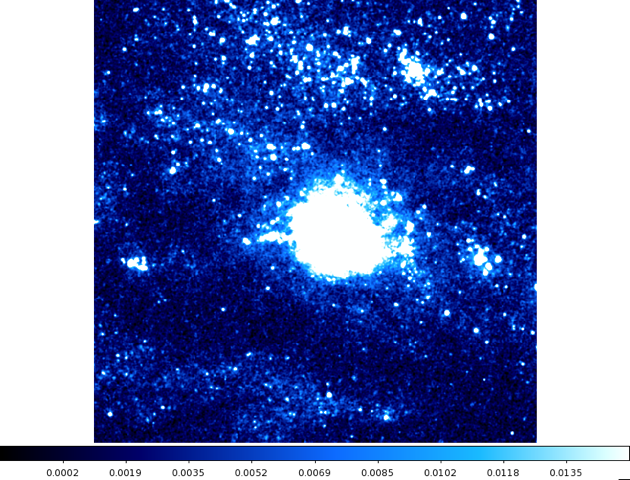
\includegraphics[width=0.52\textwidth]{small_ex.png}
    \caption{Illustration of the randomly chosen HII region for the small sample from the M83 reprojected datacube.}
    \label{img:h2region}
\end{figure}

This time, most of the experiments gave me immediate results failing or finishing. On table \ref{tab:small}, you can see the input parameters and the status of the experiments I tested with the small datacube.

\begin{table}[h!]
  \centering
    \begin{tabular}{ c c c c c c }
    \hline\hline
    
    Name & Normalized & Learning rate & Epsilon & Pruning Frequency & Status\\
    \hline
    
    ESOMtrain1 & 0 & 0.5 & 0.001 & 50 & Running\\
    Train2 & 1 & 0.5 & 0.0001 & 50 & Ended\\
    Train3 & 1 & 0.5 & 0.1 & 50 & Ended\\
    Train4 & 0 & 0.5 & 0.0001 & 50 & Running\\
    Train5 & 0 & 0.95 & 0.0001 & 100 & Running\\
    Train6 & 1 & 0.99 & 0.001 & 50 & Ended\\

    \hline
  \end{tabular}
  \caption{All the mentioned experimend belong to the SmallDataCube workspace, have 3 as data type and one input node, no previous configuration file and the input file is \emph{rp\_small\_datacube.fits}.}
  \label{tab:small}
\end{table}
In this case three of the experiments ended and none od them failed (yet), here I detected that the output file that contains the distributions of the clusters on every layer is missing, but we got some interesting resuts, in the next figures (\ref{img:smallended},\ref{img:matrixended}) you can apreciate better what I'm taking about.

\begin{figure}[h!]
	\centering
    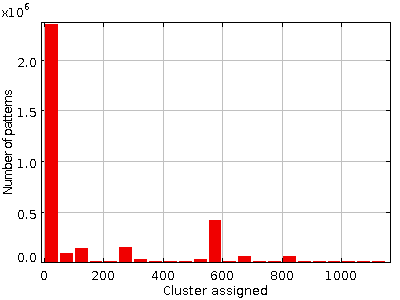
\includegraphics[width=0.31\textwidth]{Small-train2.png}
    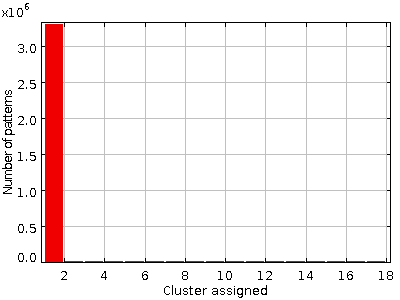
\includegraphics[width=0.31\textwidth]{Small-train3.png}
    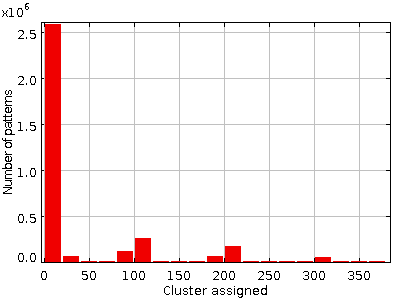
\includegraphics[width=0.31\textwidth]{Small-train6.png}
    \caption{All of the images correspond to histograms of the ended experiments mentioned above in order (Train2, Train3, Train6), as you can see there is a predominance on one of the clusters that can mean that is detecting the HII region or the experiment never started, to understand further the results a visualization of the clusters is needed.}
    \label{img:smallended}
\end{figure}

\begin{figure}[h!]
	\centering
    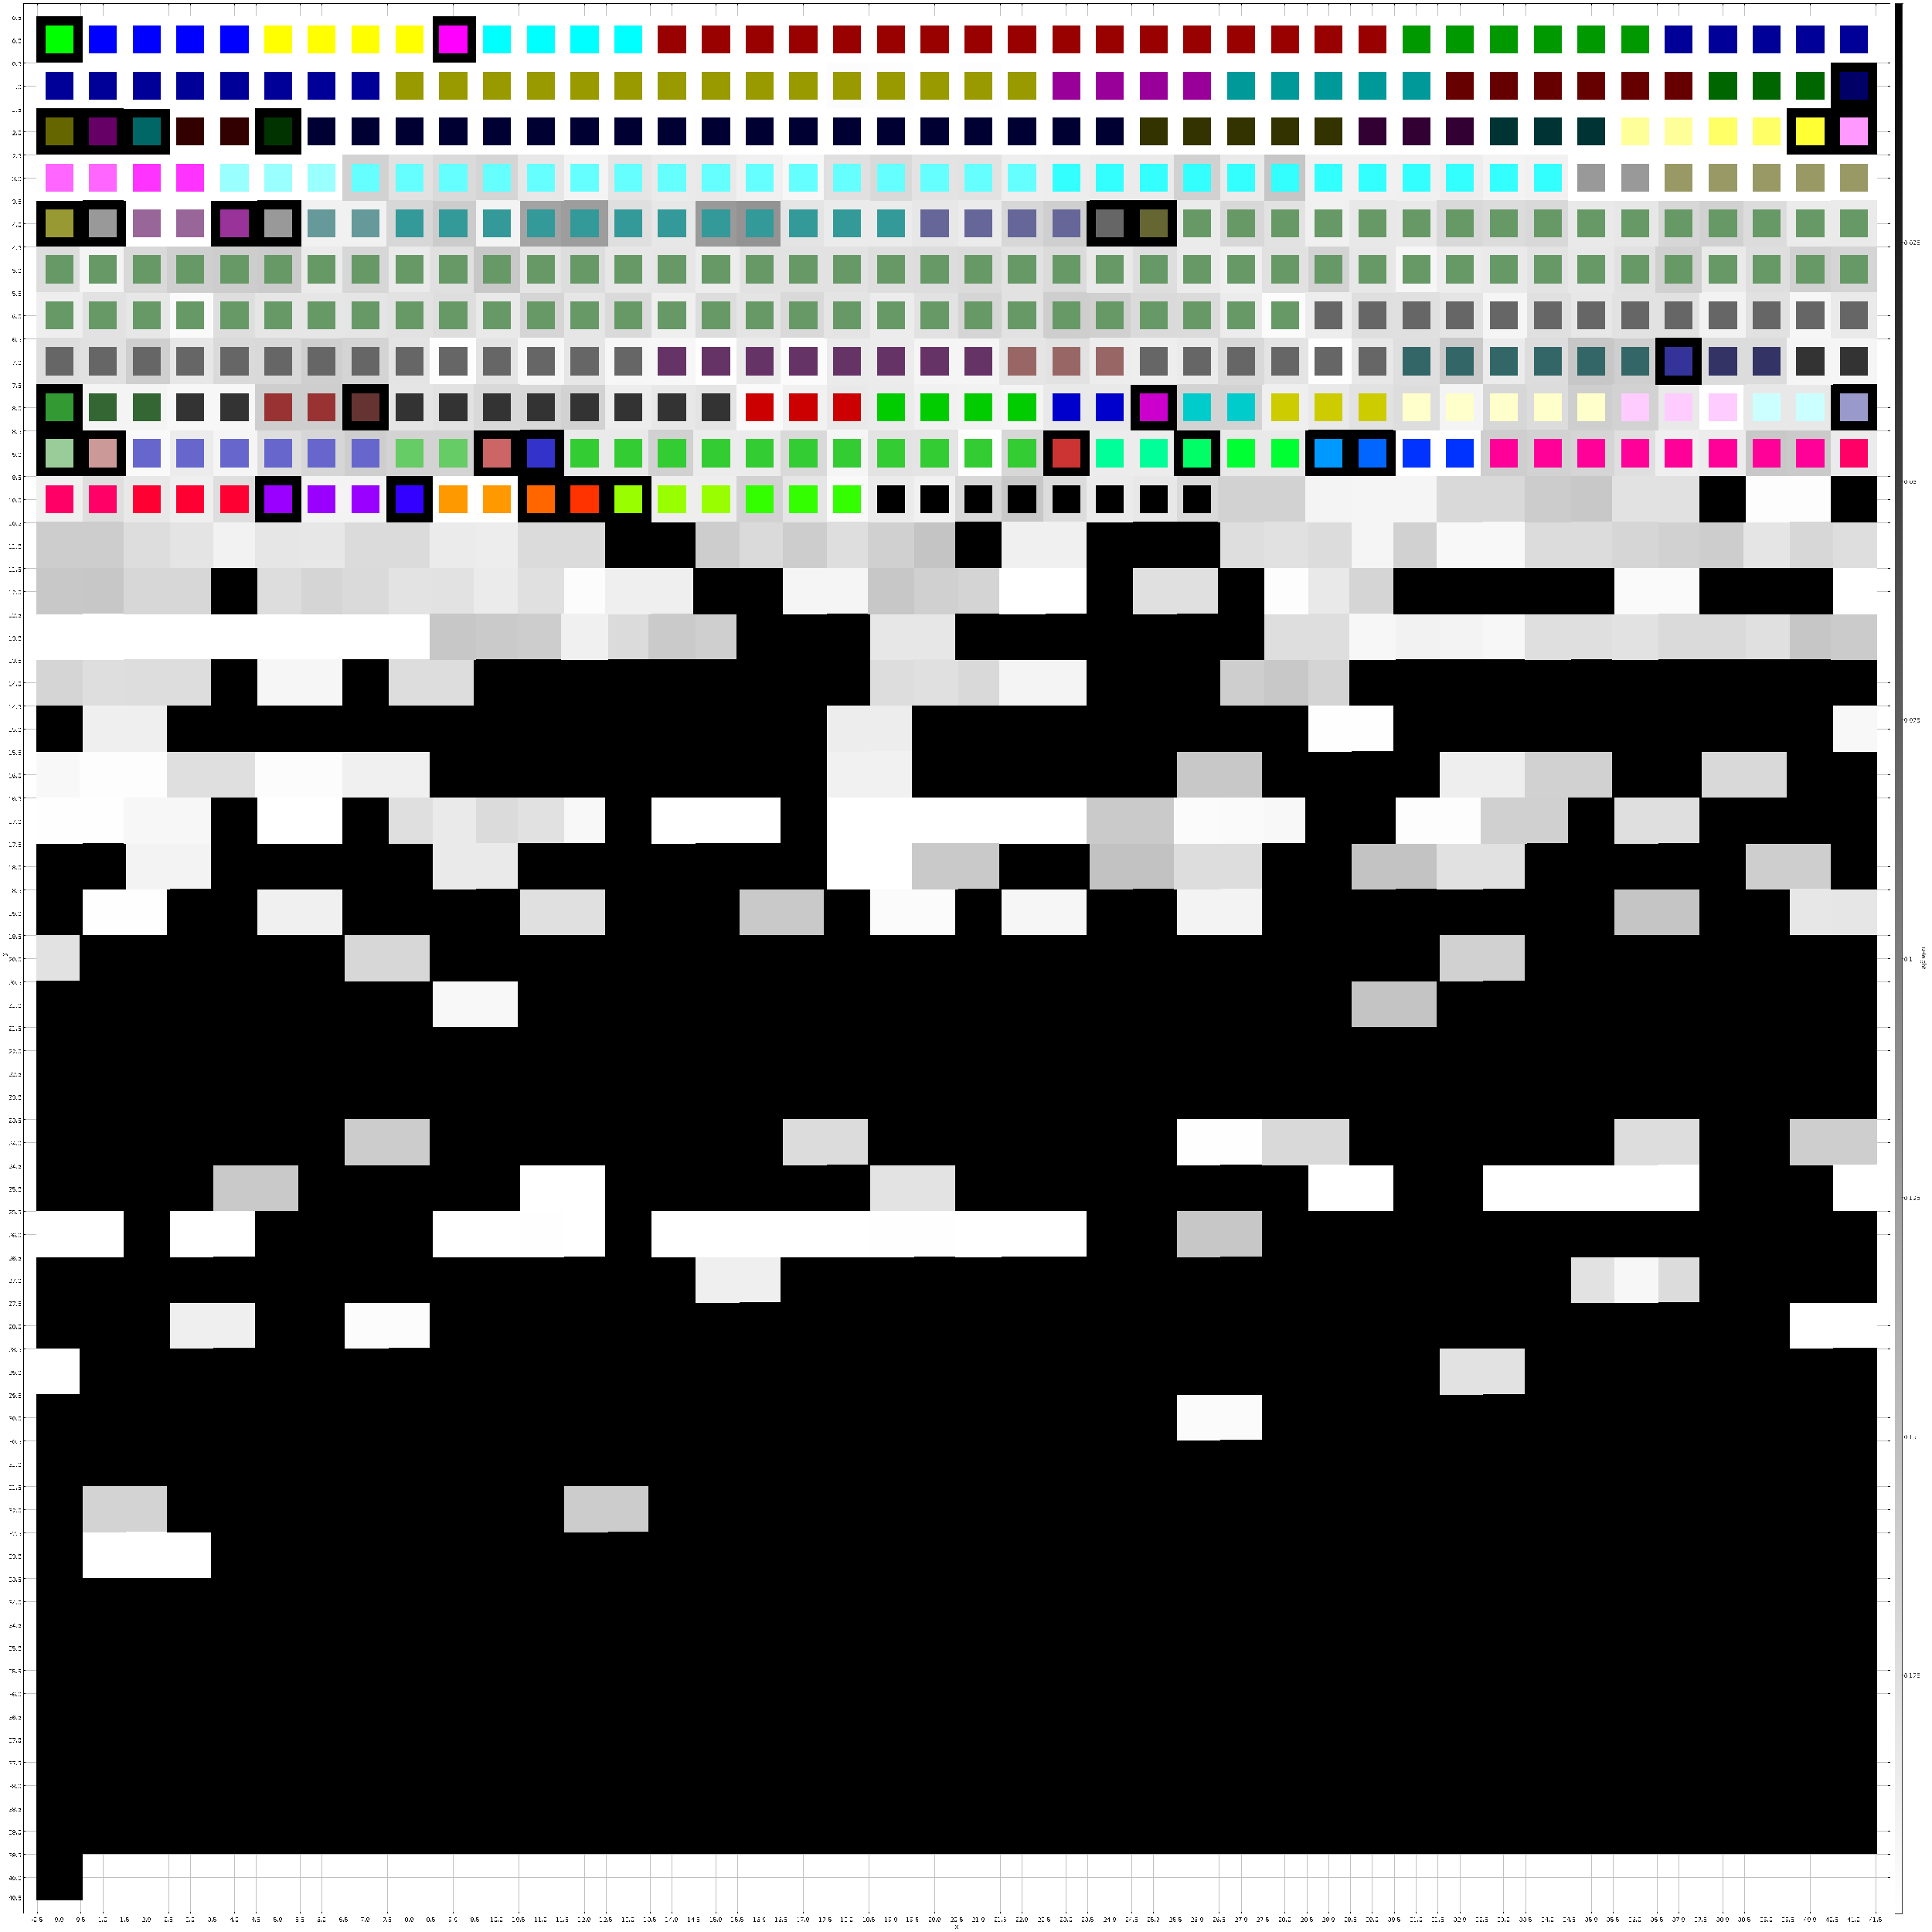
\includegraphics[width=0.31\textwidth]{matrix2-01.png}
    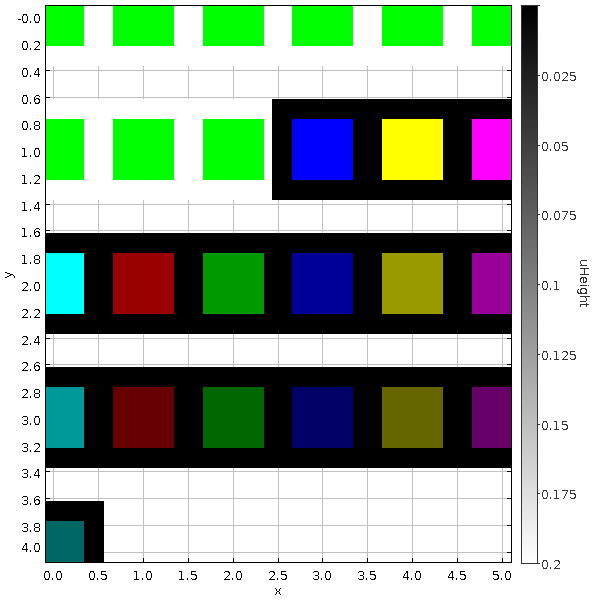
\includegraphics[width=0.31\textwidth]{Small-train3-matrix.png}
    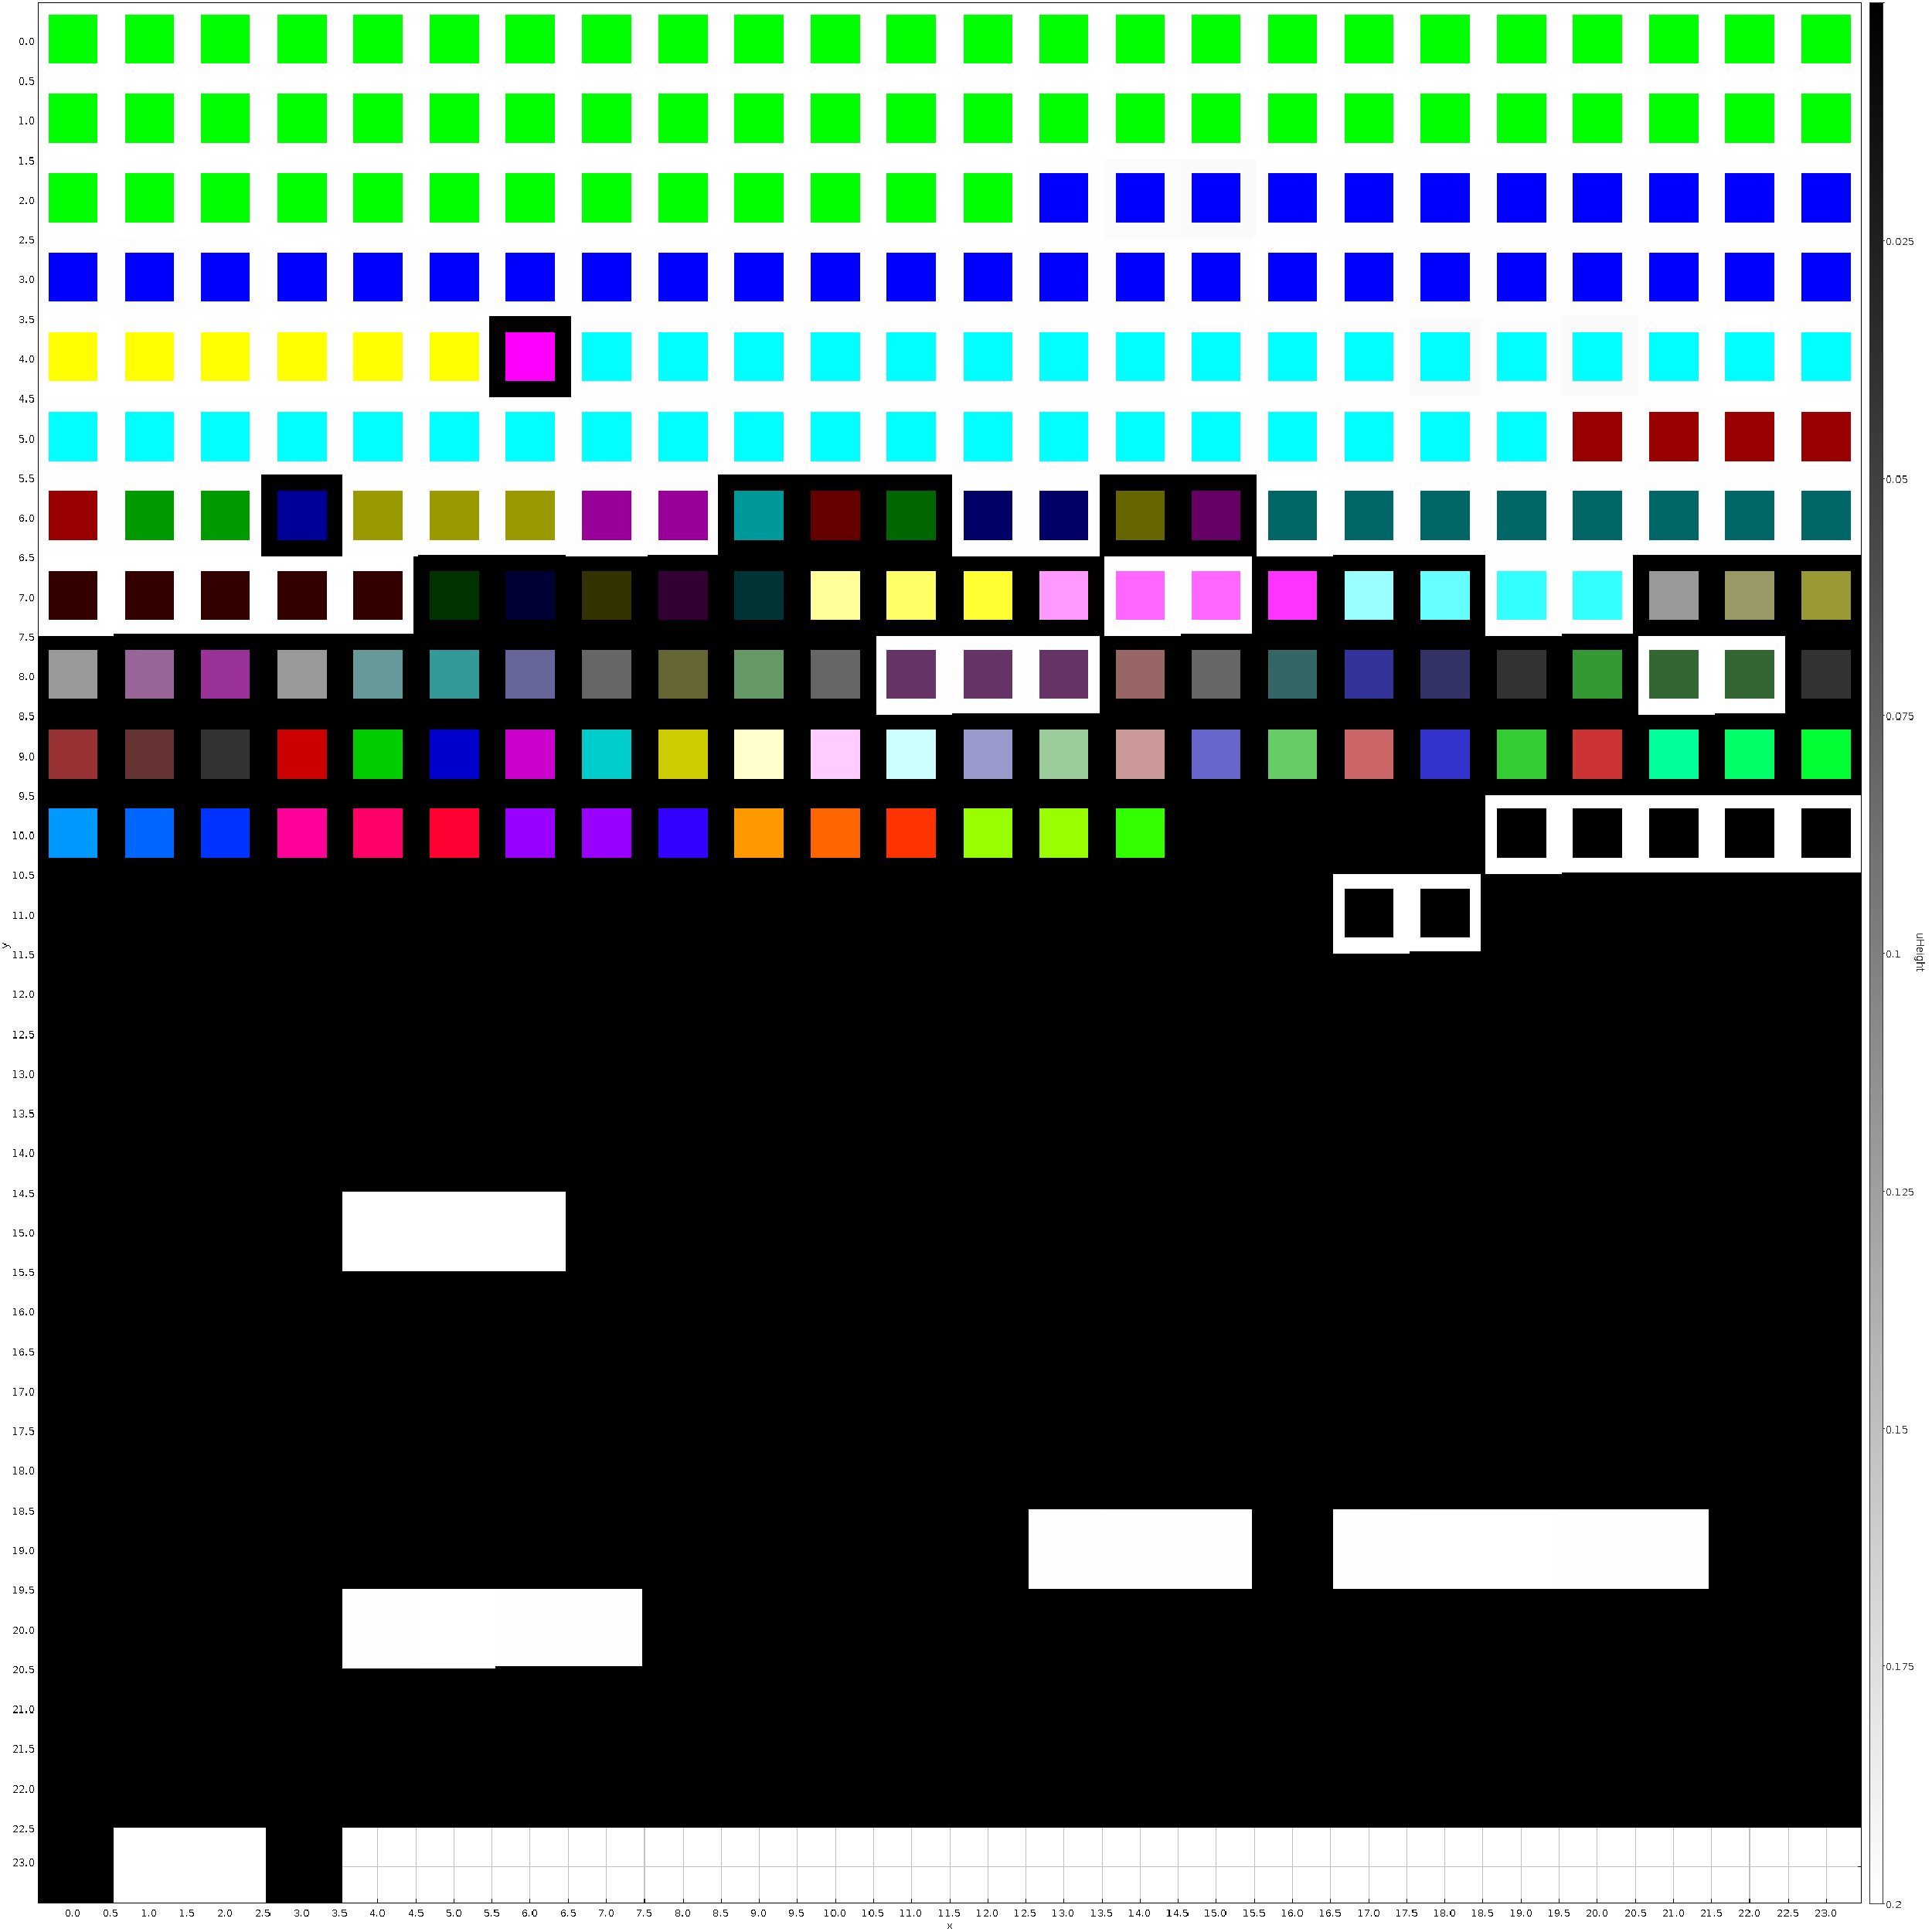
\includegraphics[width=0.31\textwidth]{matri6-01.png}
    \caption{All of the images correspond to U-matrices of the ended experiments mentioned above in order (Train2, Train3, Train6)}
    \label{img:matrixended}
\end{figure}
 There is work to be done for this cases, understand what is going on and interpret correctly the results, but last we got some.
\subsection{CSOM}
%one image
Well, as I mentioned before I did some tests using the ESOM method but since I wasn{t getting any results I thougth of testing this methond, as always I strongly recommend to read carefully its manual, \url{http://dame.dsf.unina.it/documents/SOFM_UserManual_DAME-MAN-NA-0014-Rel1.1.pdf} and fully undesrtand what is going on behind the curtains. In the meanwhile, this is my own explanation. This method uses FITS files, does not support datacubes, speciffically uses a neighborhood function in order to preserve the topological properties of the input space, it is a type of artificial network and is mainly unsupervised learning  and produces a low dimensional discretized representation of the input space of the training samples. I in this case you can choose the number of clusters/neurons in the first layer (neural network), the diameter, number of layers (in the neural network), learning rate and variance  on each layer. Here you have more input parameters to control.
\subsubsection{Expected Results}
Well in this case, since only FITS images are allowed, what we expect to find are areas indeitfying the different objects in the interstellar medium.

The important results in this case, are got in the \emph{Run} and \emph{Test} steps, in the \emph{Train} step only the network configuration is outputted. What we are interested on seein are the plotted clusters.
\subsubsection{Tests}
In this case I did some tests on the CSOM workspace, but none of the, where succesful, too many input variables to control and test. So, in this case I will leave this parameters free for you to try. I do believe that tis method could be very useful and if you find a way to input the datacube in a different configuration you will get some interesting results, due to the fact that in this method the preservation of the topology is one of the main principles.
%Mencionar los dos metodos de DAMEWARE
%Explicar los dos metodos, como untroduciste los datos, el objectivo de cada uno

%Lo que se espera obtener de cada uno de los experimentos, uno es en una sola imagen y el otro es en el datacube
%Los archivos que se obtienen y lo que significas, lo que se puede hacer



%Poner los parametros que se han elegido en los experimentos fallidos, y los que siguen en modo running
%Exlpicar por fases los experimentos que se intentaron


\section{Further work}
Well, finally we reached the point where I my time in Canada finished and I this research is still on its first stages. I have so many ideas of how to explore the clustering techniques in the DAME platform, MatLab, Python and everything else that can be tested. 

\subsection{Some interesting ideas}
%Normalizar los datos
%Acomodarlos y hacer que los paquetes sean mas pequeños
%Random points
For now, I would say that your best chance here, is to device an efficient way to input the information contained in a datacube as a list of points with values and reduce its dimensionality by randomly choosing them on every layer. If you are ever stuck, or no new ideas come to your mind, do not hesitate to contact me I might have a new interesting idea you can test.

\subsection{Links you should check out}
Most of them are listed in the useful resourses section of The Caltech-JPL Summer School on Big Data Analytics, the webpage \url{https://class.coursera.org/bigdataschool-001/wiki/Useful_resources}, you may need to create an account in Coursera and enroll in the course. And the rest of them are located in the References section on my GitHub page, \url{https://github.com/LaurethTeX/Clustering/blob/master/References.md}.
%Los links que estan en la pagina de el curso de caltech
%Sky surveys
%MATLAB SOM toolbox
%SAO datamining
\vfill
\textit{Wish you all the best, Andrea Hidalgo}
\end{document}